\documentclass{beamer}

\usepackage{amsmath,amsfonts}
\usepackage{bm}
\usepackage{nicefrac}
\usepackage{mathrsfs}
\usepackage{etex}
\usepackage{ccicons}
\usepackage{pgfplots,tikz}
\usepackage{tikz-qtree}
\usepackage{algorithms/algorithm}
\usepackage{algorithms/algorithmic}
\usepackage[T1]{fontenc}
\usepackage{cancel}
\usepackage{xcolor}
\usepackage{rotating}


\newlength\figureheight
\newlength\figurewidth

\definecolor{gray}{gray}{0.4}

\makeatletter
\@ifclassloaded{beamer}{
\usefonttheme[onlymath]{serif}
\uselanguage{French}
\languagepath{French}
% Git hash
\usepackage{xstring}
\usepackage{catchfile}
\immediate\write18{git rev-parse HEAD > git.hash}
\CatchFileDef{\HEAD}{git.hash}{\endlinechar=-1}
\newcommand{\gitrevision}{\StrLeft{\HEAD}{7}}
}{}
\makeatother

\makeatletter
\@ifclassloaded{beamer}{
\setbeamertemplate{footline}{
  {\hfill\vspace*{1pt}\href{https://creativecommons.org/publicdomain/zero/1.0/legalcode.en}{\ccZero}\hspace{.1cm}
    \href{https://mnemosyne.ithaca.fr/stephane/ep-mj-30-years/blob/\HEAD/tex/slides/sep.tex}{\gitrevision}\enspace--\enspace\today\enspace
  }}}
\makeatother

\makeatletter
\newenvironment{sqcases}{%
  \matrix@check\sqcases\env@sqcases
}{%
  \endarray\right.%
}
\def\env@sqcases{%
  \let\@ifnextchar\new@ifnextchar
  \left\lbrack
  \def\arraystretch{1.2}%
  \array{@{}l@{\quad}l@{}}%
}
\makeatother


\begin{document}

\setbeamertemplate{navigation symbols}{}


\title{The stochastic extended path approach}
\author{St\'ephane Adjemian\footnote{Universit\'e du Mans, Dynare team} and Michel Juillard\footnote{Dynare team}}
\date{February, 2025}

\begin{frame}
  \titlepage{}
\end{frame}


\begin{frame}
  \frametitle{Motivations}

  \begin{itemize}

  \item Nonlinearities can play an important role in macroeconomics:
    Irreversible investment, ZLB, Borrowing constraint, \ldots\newline

  \item Standard local approximation techniques fail to produce
    reliable results in the presence of kinks.\newline

  \item Deterministic, perfect forresight models can be solved with much
    greater accuracy than stochastic ones.\newline

  \item The extended path approach aims to leverage the accuracy of
    deterministic methods in capturing (deterministic) nonlinearities.\newline

  \item But it neglects the implications of future uncertainty. Is
    this a concern? Can we improve the EP approach?

  \end{itemize}
\end{frame}


\begin{frame}
\frametitle{Model to be solved}

\[
\mathbb E_t\left[ f\left( y_{t-1},y_t,y_{t+1},\varepsilon_t \right) \right] = 0
\]

\bigskip

\begin{itemize}

\item $y$ an $n\times 1$ vector of endogenous variables\newline

\item $f: \mathbb R^{3n+q}\rightarrow \mathbb R^n$\newline

\item $\varepsilon_t \sim \mathcal N\left( 0,\Sigma \right) \perp y_{\underline{t-1}}$\newline

\item $ \exists\, y^{\star}$ such that $f\left( y^{\star},y^{\star},y^{\star},0 \right)=0$

\end{itemize}

\end{frame}


\begin{frame}
  \frametitle{Perfect foresight version}

  \[
    \begin{cases}
      f\left( {\color{red}y_{t-1}},y_t,y_{t+1},\varepsilon_t \right) = 0\\
      f\left( y_{t+h-1},y_{t+h},y_{t+h+1}, 0 \right) = 0\quad \text{ for }h=1,\ldots,H-2\\
      f\left( y_{t+H-2},y_{t+H-1},{\color{red}y^{\star}}, 0 \right) = 0\\
    \end{cases}
  \]


  \begin{itemize}
  \item Perfect foresight models, after a shock economy returns asymptotically
    to equilibirum.
  \item For a long enough simulation, one can consider that for all
    practical purpose the system is back to equilibrium.
  \item This suggests to solve a two value boundary problem with
    initial conditions for some variables (backward looking) and
    terminal conditions for others (forward looking).
  \item In practice, one can use a Newton method to the equations of
    the model stacked over all periods of the simulation.
  \item The Jacobian matrix of the stacked system is very sparse and
    this characteristic must be used to write a practical algorithm.
  \end{itemize}

\end{frame}


\begin{frame}
  \frametitle{Solve perfect foresight models}
\end{frame}


\begin{frame}
  \frametitle{Stochastic perfect foresight models}
\end{frame}


\begin{frame}[c]{}
  \frametitle{Stochastic perfect foresight models}
  \framesubtitle{order 1}
  \centering
  \[
    \begin{split}
      &\sum_{i=1}^n\omega_i f\left( y_{i,t+1}, {\color{red} y_t}, {\color{blue} y_{t-1}}\right) = 0\\
      \begin{sideways}\hspace{-.6cm}\footnotesize{i=1,\dots,n}\end{sideways} &\begin{sqcases}
        f\left( y_{i,t+2}, y_{i,t+1}, {\color{red}y_t}, \epsilon_i \right) = 0\\
        f\left( y_{i,t+3}, y_{i,t+2}, y_{i,t+1}, 0 \right) = 0\\
        \vdots\\
        f\left( {\color{blue}y^{\star}}, y_{i,t+H-1}, y_{i,t+H-2}, 0 \right) = 0\\
      \end{sqcases}
    \end{split}
  \]

\end{frame}


\begin{frame}[c,fragile]{}
  \frametitle{Stochastic perfect foresight models}
  \framesubtitle{order 1}
  \centering

  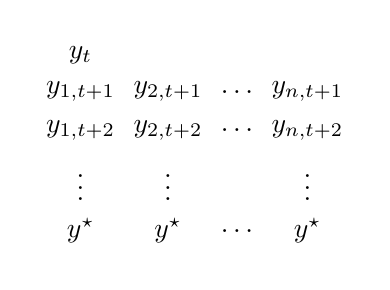
\begin{tikzpicture}
\matrix
  {
    \node {$y_t$}; & \node{}; & \node {}; & \node {}; \\
    \node {$y_{1,t+1}$}; & \node{$y_{2,t+1}$}; & \node{$\ldots$};& \node{$y_{n,t+1}$}; \\
    \node {$y_{1,t+2}$}; & \node{$y_{2,t+2}$}; & \node{$\ldots$};& \node{$y_{n,t+2}$}; \\
    \node {$\vdots$}; & \node{$\vdots$}; & \node{};& \node{$\vdots$}; \\
    \node {$y^\star$}; & \node{$y^\star$}; & \node{$\ldots$};& \node{$y^\star$}; \\
  };
\end{tikzpicture}

\end{frame}



\begin{frame}
  \frametitle{Stochastic perfect foresight model}
  \framesubtitle{Stacked jacobian, order=1, three nodes}
  \begin{center}
    \scalebox{.5}{
  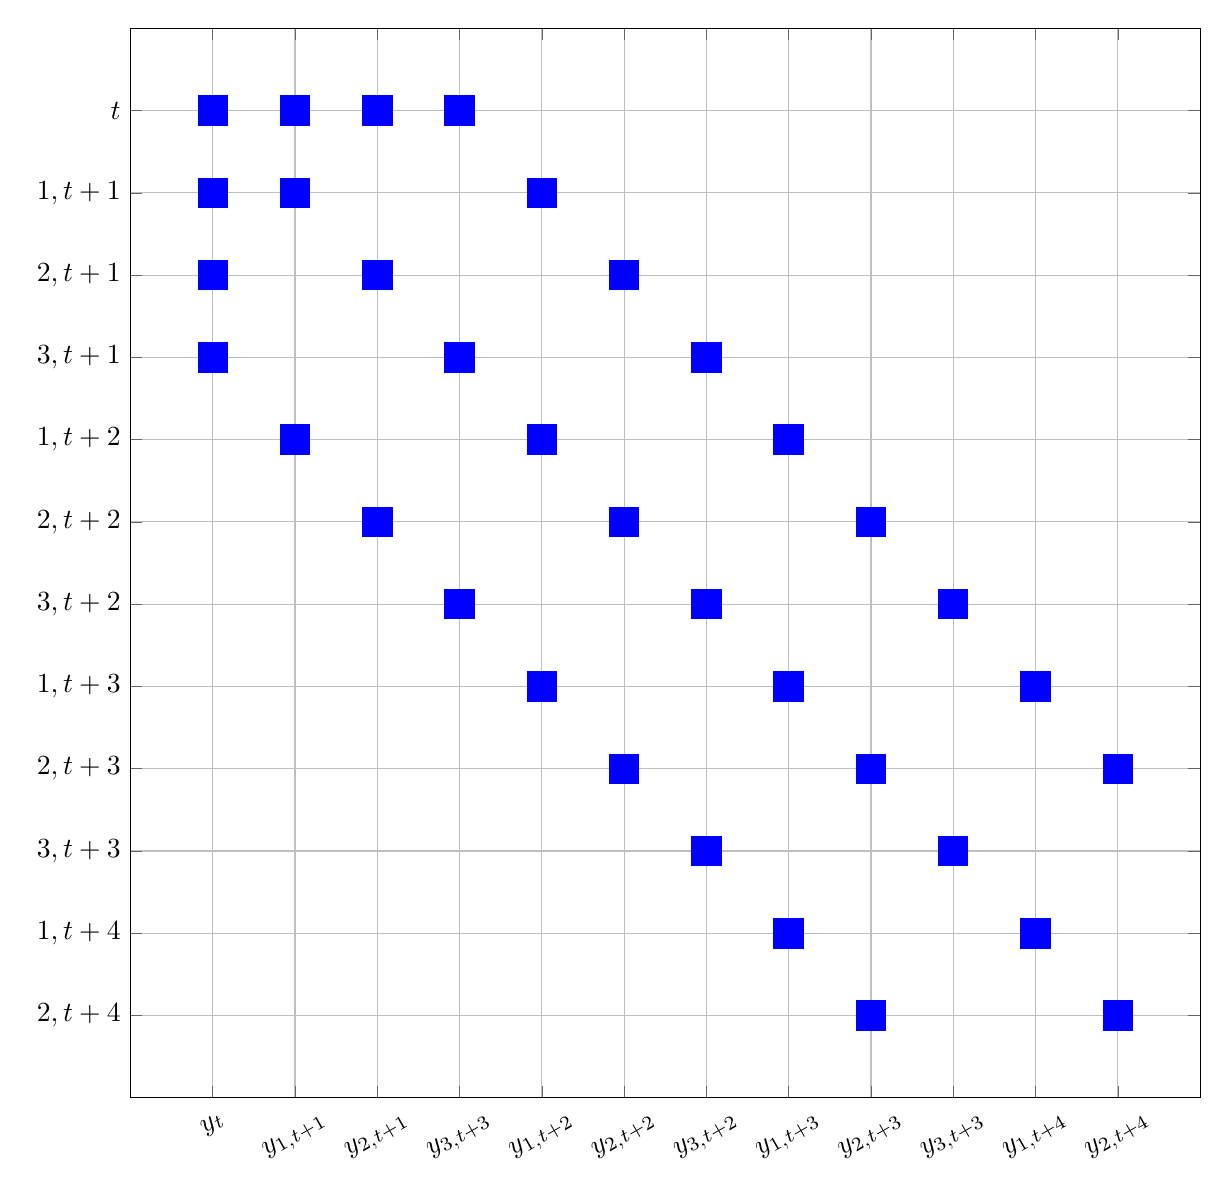
\begin{tikzpicture}

\begin{axis}[%
width=5.348in,
height=5.348in,
at={(1.854in,0.722in)},
scale only axis,
xmin=0,
xmax=13,
xtick={1,2,3,4,5,6,7,8,9,10,11,12},
xticklabels={$y_t$,$y_{1,t+1}$,$y_{2,t+1}$,$y_{3,t+3}$,$y_{1,t+2}$,$y_{2,t+2}$,$y_{3,t+2}$,$y_{1,t+3}$,$y_{2,t+3}$,$y_{3,t+3}$,$y_{1,t+4}$,$y_{2,t+4}$},
xticklabel style={rotate=30},
y dir=reverse,
ymin=0,
ymax=13,
ytick={1,2,3,4,5,6,7,8,9,10,11,12},
yticklabels={$t$,{$1,t+1$},{$2,t+1$},{$3,t+1$},{$1,t+2$},{$2,t+2$},{$3,t+2$},{$1,t+3$},{$2,t+3$},{$3,t+3$},{$1,t+4$},{$2,t+4$}},
axis background/.style={fill=white},
xmajorgrids,
ymajorgrids
]
\addplot [color=blue, only marks, mark size=5.3pt, mark=square*, mark options={solid, blue}, forget plot]
  table[row sep=crcr]
  \end{center}
\end{frame}


  \begin{frame}[c]{}
  \frametitle{Stochastic perfect foresight models}
  \framesubtitle{order 2}
  \centering

  \[
    \begin{split}
      &\sum_{i=1}^n\omega_i f\left( y_{i,t+1}, {\color{red} y_t}, {\color{blue} y_{t-1}}\right) = 0\\
      \begin{sideways}\hspace{-.6cm}\footnotesize{i=1,\dots,n}\end{sideways} & \begin{sqcases}
        \sum_{j=1}^n\omega_jf\left( y_{j,i,t+2}, y_{i,t+1}, {\color{red}y_t}, \epsilon_i \right) = 0\\
        \begin{sideways}\hspace{-.6cm}\footnotesize{j=1,\dots,n}\end{sideways} \begin{sqcases}
          f\left( y_{j,i,t+3}, y_{j,i,t+2}, y_{i,t+1}, \epsilon_j \right) = 0\\
          f\left( y_{j,i,t+4}, y_{j,i,t+3}, y_{j,i,t+2}, 0 \right) = 0\\
          \vdots\\
          f\left( {\color{blue}y^{\star}}, y_{j,i,t+H-1}, y_{j,i,t+H-2}, 0 \right) = 0
        \end{sqcases}
      \end{sqcases}
    \end{split}
  \]

  \end{frame}


  \begin{frame}[c,fragile]{}
  \frametitle{Stochastic perfect foresight models}
  \framesubtitle{order 2}
  \centering

  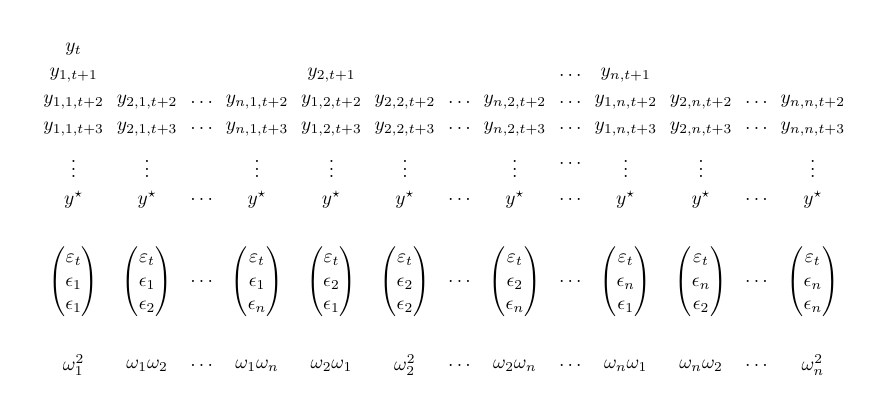
\begin{tikzpicture}[scale=0.7, every node/.style={scale=0.7}]
\matrix
  {
    \node {$y_t$}; & \node{}; & \node {}; & \node {}; \node {}; & \node{}; & \node {}; & \node {}; & \node{}; & \node{}; & \node {}; & \node {}; & \node{};\\
    \node {$y_{1,t+1}$}; & \node{}; & \node{}; & \node{}; & \node {$y_{2,t+1}$}; & \node{}; & \node{}; & \node{}; & \node{$\ldots$}; & \node {$y_{n,t+1}$}; & \node{}; & \node{}; & \node{}; \\
    \node {$y_{1,1,t+2}$}; & \node{$y_{2,1,t+2}$}; & \node{$\ldots$}; & \node{$y_{n,1,t+2}$}; & \node {$y_{1,2,t+2}$}; & \node{$y_{2,2,t+2}$}; & \node{$\ldots$}; & \node{$y_{n,2,t+2}$}; & \node{$\ldots$}; & \node {$y_{1,n,t+2}$}; & \node{$y_{2,n,t+2}$}; & \node{$\ldots$};& \node{$y_{n,n,t+2}$}; \\
    \node {$y_{1,1,t+3}$}; & \node{$y_{2,1,t+3}$}; & \node{$\ldots$}; & \node{$y_{n,1,t+3}$}; & \node {$y_{1,2,t+3}$}; & \node{$y_{2,2,t+3}$}; & \node{$\ldots$};& \node{$y_{n,2,t+3}$}; & \node{$\ldots$}; & \node {$y_{1,n,t+3}$}; & \node{$y_{2,n,t+3}$}; & \node{$\ldots$};& \node{$y_{n,n,t+3}$};\\
    \node {$\vdots$}; & \node{$\vdots$}; & \node{};& \node{$\vdots$}; & \node {$\vdots$}; & \node{$\vdots$}; & \node{};& \node{$\vdots$}; & \node{$\ldots$}; & \node {$\vdots$}; & \node{$\vdots$}; & \node{};& \node{$\vdots$};\\
    \node {$y^\star$}; & \node{$y^\star$}; & \node{$\ldots$};& \node{$y^\star$}; & \node {$y^\star$}; & \node{$y^\star$}; & \node{$\ldots$};& \node{$y^\star$}; & \node{$\ldots$}; & \node {$y^\star$}; & \node{$y^\star$}; & \node{$\ldots$};& \node{$y^\star$};\\
\node {}; & \node{}; & \node{};& \node{}; & \node {}; & \node{}; & \node{};& \node{}; & \node{}; & \node {}; & \node{}; & \node{};& \node{};\\
\node {}; & \node{}; & \node{};& \node{}; & \node {}; & \node{}; & \node{};& \node{}; & \node{}; & \node {}; & \node{}; & \node{};& \node{};\\
\node {$\begin{pmatrix}\varepsilon_t\\ \epsilon_1 \\ \epsilon_1\end{pmatrix}$}; & \node{$\begin{pmatrix}\varepsilon_t\\ \epsilon_1 \\ \epsilon_2\end{pmatrix}$}; & \node{$\ldots$};& \node{$\begin{pmatrix}\varepsilon_t\\ \epsilon_1 \\ \epsilon_n\end{pmatrix}$}; & \node {$\begin{pmatrix}\varepsilon_t\\ \epsilon_2 \\ \epsilon_1\end{pmatrix}$}; & \node{$\begin{pmatrix}\varepsilon_t\\ \epsilon_2 \\ \epsilon_2\end{pmatrix}$}; & \node{$\ldots$};& \node{$\begin{pmatrix}\varepsilon_t\\ \epsilon_2 \\ \epsilon_n\end{pmatrix}$}; & \node{$\ldots$}; & \node {$\begin{pmatrix}\varepsilon_t\\ \epsilon_n \\ \epsilon_1\end{pmatrix}$}; & \node{$\begin{pmatrix}\varepsilon_t\\ \epsilon_n \\ \epsilon_2\end{pmatrix}$}; & \node{$\ldots$};& \node{$\begin{pmatrix}\varepsilon_t\\ \epsilon_n \\ \epsilon_n\end{pmatrix}$};\\
\node {}; & \node{}; & \node{};& \node{}; & \node {}; & \node{}; & \node{};& \node{}; & \node{}; & \node {}; & \node{}; & \node{};& \node{};\\
\node {}; & \node{}; & \node{};& \node{}; & \node {}; & \node{}; & \node{};& \node{}; & \node{}; & \node {}; & \node{}; & \node{};& \node{};\\
\node {$\omega_1^2$}; & \node{$\omega_1\omega_2$}; & \node{$\ldots$};& \node{$\omega_1\omega_n$}; & \node {$\omega_2\omega_1$}; & \node{$\omega_2^2$}; & \node{$\ldots$};& \node{$\omega_2\omega_n$}; & \node{$\ldots$}; & \node {$\omega_n\omega_1$}; & \node{$\omega_n\omega_2$}; & \node{$\ldots$};& \node{$\omega_n^2$};\\
  };
\end{tikzpicture}

\end{frame}


\begin{frame}
    \frametitle{Stochastic perfect foresight model}
    \framesubtitle{Stacked jacobian, order=2, three nodes}
  \begin{center}
    \scalebox{.5}{
  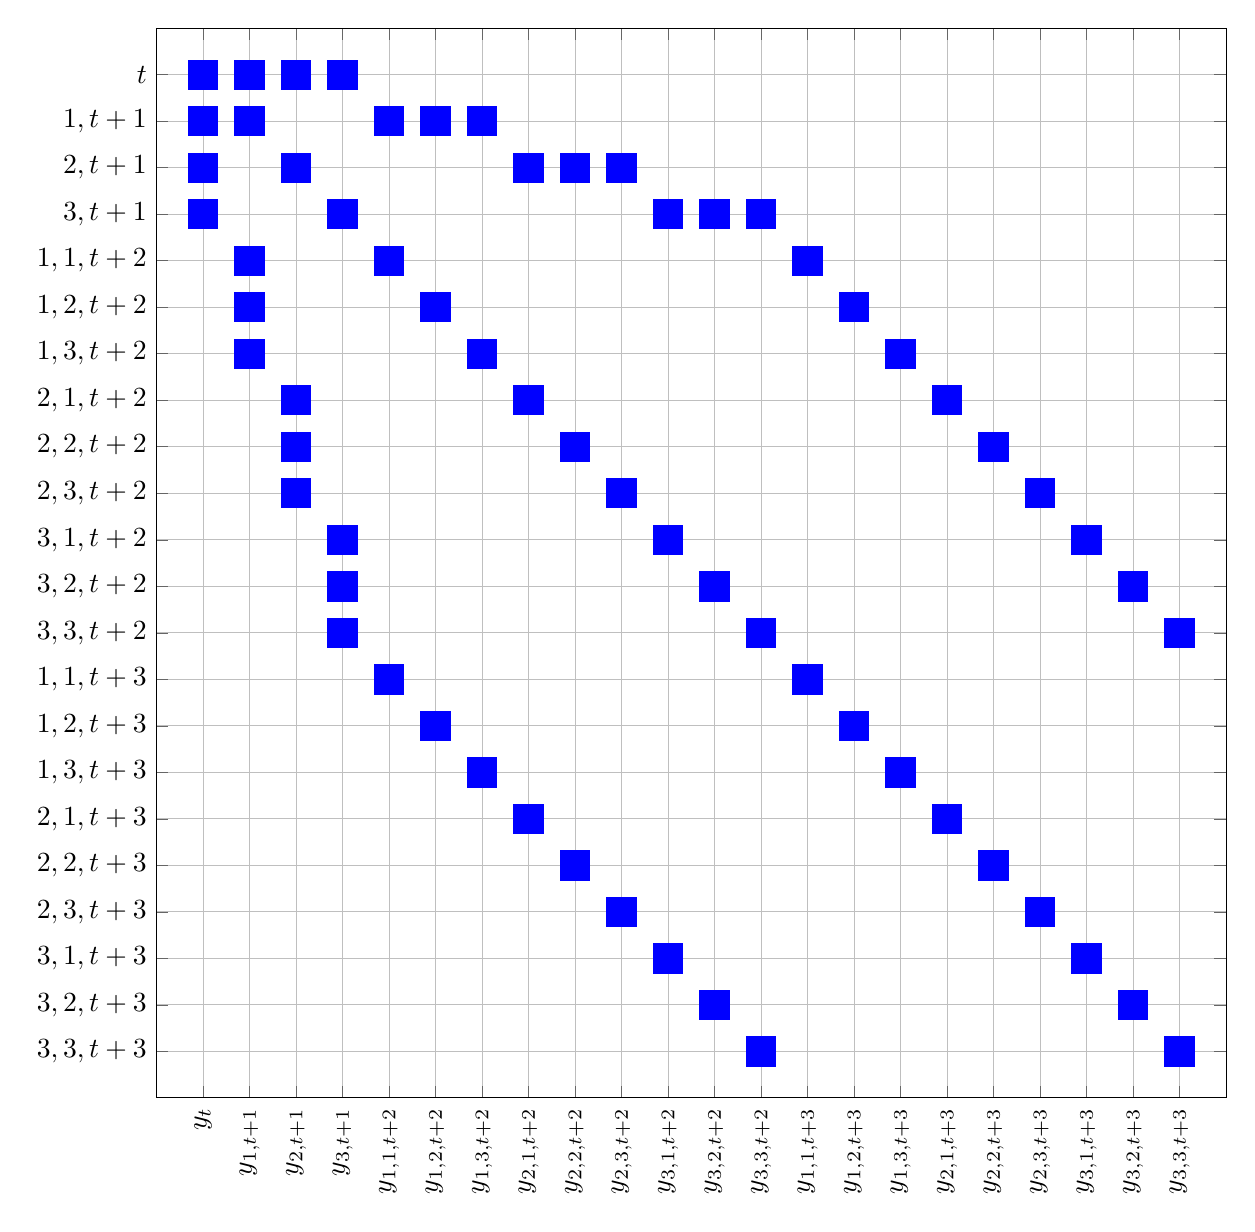
\begin{tikzpicture}

\begin{axis}[%
width=5.348in,
height=5.348in,
at={(1.854in,0.722in)},
scale only axis,
xmin=0,
xmax=23,
xtick={1,2,3,4,5,6,7,8,9,10,11,12,13,14,15,16,17,18,19,20,21,22},
xticklabels={{$y_t$},{$y_{1,t+1}$},{$y_{2,t+1}$},{$y_{3,t+1}$},{$y_{1,1,t+2}$},{$y_{1,2,t+2}$},{$y_{1,3,t+2}$},{$y_{2,1,t+2}$},{$y_{2,2,t+2}$},{$y_{2,3,t+2}$},{$y_{3,1,t+2}$},{$y_{3,2,t+2}$},{$y_{3,3,t+2}$},{$y_{1,1,t+3}$},{$y_{1,2,t+3}$},{$y_{1,3,t+3}$},{$y_{2,1,t+3}$},{$y_{2,2,t+3}$},{$y_{2,3,t+3}$},{$y_{3,1,t+3}$},{$y_{3,2,t+3}$},{$y_{3,3,t+3}$}},
xticklabel style={rotate=90},
y dir=reverse,
ymin=0,
ymax=23,
ytick={1,2,3,4,5,6,7,8,9,10,11,12,13,14,15,16,17,18,19,20,21,22},
yticklabels={$t$,{$1,t+1$},{$2,t+1$},{$3,t+1$},{$1,1,t+2$},{$1,2,t+2$},{$1,3,t+2$},{$2,1,t+2$},{$2,2,t+2$},{$2,3,t+2$},{$3,1,t+2$},{$3,2,t+2$},{$3,3,t+2$},{$1,1,t+3$},{$1,2,t+3$},{$1,3,t+3$},{$2,1,t+3$},{$2,2,t+3$},{$2,3,t+3$},{$3,1,t+3$},{$3,2,t+3$},{$3,3,t+3$}},
axis background/.style={fill=white},
xmajorgrids,
ymajorgrids
]
\addplot [color=blue, only marks, mark size=5.3pt, mark=square*, mark options={solid, blue}, forget plot]
  table[row sep=crcr]
  \end{center}

\end{frame}


\begin{frame}
  \frametitle{Burnside (1998) asset pricing model}

\begin{itemize}

  \item The price/dividend ratio and the growth rate of dividends:
  \[
    \begin{split}
      y_t &= \beta \mathbb E_t\left[e^{\theta x_{t+1}}\left(1+y_{t+1}\right)\right]\\
      x_t &= (1-\rho)\bar x + \rho x_{t-1}+\epsilon_t
    \end{split}
  \]

  \item The exact solution is:
\[
    y_t = \sum_{i=1}^\infty \beta^i e^{a_i+b_i\hat x_t}
\]
where
\[
    a_i = \theta \bar x i +
\frac{\theta^2\sigma^2}{2(1-\rho)^2}\left(i-2\rho\frac{1-\rho^i}{1-\rho}+\rho^2\frac{1-\rho^{2i}}{1-\rho^2}\right)
\]
and
\[
b_i = \frac{\theta\rho\left(1-\rho^i\right)}{1-\rho}
\]

\end{itemize}

\end{frame}


\begin{frame}
  \frametitle{Numerical simulation}
   \framesubtitle{Calibration}

\begin{align*}
  \bar x &= 0.0179\\
  \rho &=  -0.139\\
  \theta &= -1.5\\
  \beta &= 0.95\\
  \sigma &= 0.0348\\
\end{align*}

\medskip

\begin{itemize}
\item The deterministic steady state is equal to 12.3035.\newline
\item The risky steady state, defined as the fix point in absence of
  shock this period:
\[
\widetilde y = \sum_{i=1}^\infty \beta^i e^{\theta \bar x i +
\frac{\theta^2\sigma^2}{2(1-\rho)^2}\left(i-2\rho\frac{1-\rho^i}{1-\rho}+\rho^2\frac{1-\rho^{2i}}{1-\rho^2}\right)}\approx 12.4812
\]

\end{itemize}

\end{frame}

\begin{frame}
\frametitle{Comparing SEP, perturbation and closed-form solution}

Simulate long time series ($T=8000$) and compare with true solution. We use a quadrature with 3 nodes for SEP.\newline

\bigskip

\begin{tabular}{l|cc|cc}
  \hline
  & P(1) & P(2) & SEP(0) & SEP(2)\\ \hline
  $100\times\textrm{mean}(|\hat y_t - y_t|/y_t)$  & 1.4261 &  0.0193 & 1.4241 &  1.2534\\
  $100\times\textrm{max}(|\hat y_t - y_t|/y_t)$   & 1.4707 &  0.0527 & 1.4250 &  1.2539\\ \hline\hline
\end{tabular}

\bigskip\bigskip

One can show, using the closed for solution and considering an infinite number of weights and nodes in the quadrature, that we would have to consider an approximation order greater than 60, to be able to recover the theoretical mean of the price-dividend ratio.


\end{frame}



\begin{frame}
  \frametitle{Hybrid approach}

\begin{itemize}

  \item Consider a Taylor expansion of the original problem only along the scale $\sigma$ of the shocks\newline

  \item Use the second order correction for the constant.\newline

  \item[$\Rightarrow$] For K-order SEP, replace $y_{t+K+1}$ in the equations in period $K$ by $y_{t+K+1}+\frac{1}{2}g_{\sigma\sigma}$.\newline

\end{itemize}

\bigskip

\scalebox{.9}{
\begin{tabular}{l|c|ccc}
  \hline
  & P(2) & SEP(2) & SEP(2+) & SEP(10+)\\ \hline
  $100\times\textrm{mean}(|\hat y_t - y_t|/y_t)$  & 0.0193 & 1.2534 & 0.0165 & 0.0153\\
  $100\times\textrm{max}(|\hat y_t - y_t|/y_t)$   & 0.0527 & 1.2539 & 0.0179 & 0.0170\\ \hline\hline
\end{tabular}}

\end{frame}


\begin{frame}
  \frametitle{Irreversible investment}
Consider the following RBC model with irreversible investment:
\[
  \begin{split}
    \max_{\{c_{t+j},l_{t+j},k_{t+j+1}\}_{j=0}^{\infty}} &\quad \mathcal W_t = \sum_{j=0}^{\infty}\beta^ju(c_{t+j},l_{t+j})\\
           \underline{s.t.}   &  \\
              \qquad y_t &= c_t + i_t\\
              \qquad y_t &= A_tf(k_{t},l_t)\\
              \qquad k_{t+1} &= i_t + (1-\delta)k_{t}\\
              \qquad A_{t} &= {A^{\star}}e^{a_{t}}\\
              \qquad a_{t} &= \rho a_{t-1} + \varepsilon_t\\
              \qquad i_t &\ge 0
  \end{split}
\]
\end{frame}

\begin{frame}
\frametitle{Further specifications}
The utility function is
\[
  u(c_t,l_t) = \frac{\left(c_t^{\theta}(1-l_t)^{1-\theta}\right)^{\tau}}{1-\tau}
\]
and the production function,
\[
  f(k_{t},l_t) = \left(\alpha k_{t}^{\psi} + (1-\alpha)l_t^{\psi}\right)^{\frac{1}{\psi}}
\]
\end{frame}

\begin{frame}
\frametitle{First order conditions}
{\footnotesize\[
\begin{split}
  u_c(c_t,l_t) - \mu_t &= \beta \mathbb E_t\Big[
    u_c(c_{t+1},l_{t+1})\Bigl(A_{t+1}f_k(k_{t+1},l_{t+1}) + 1
    -\delta\Bigr) - \mu_{t+1}(1-\delta)\Big]\\
  \frac{u_{l}(c_t,l_t)}{u_c(c_t,l_t)} &= A_tf_l(k_t,l_t)\\
  c_t + k_{t+1} &= A_tf(k_{t},l_t) + (1-\delta)k_{t}\\
  0 &= \mu_t \left( k_{t+1} - (1-\delta)k_{t} \right)
\end{split}
\]}

\bigskip\bigskip

where $\mu_t$ is the Lagrange multiplier associated with the constraint on investment.
\end{frame}

\begin{frame}
  \frametitle{Calibration}
  \begin{align*}
    \beta    &=  0.990\\
    \theta   &=  0.357\\
    \tau     &=  2.000\\
    \alpha   &=  0.450\\
    \psi     &= -0.500\\
    \delta   &=  0.010\\
    \rho     &=  0.800\\
    A^\star &=  1.000\\
    \sigma   &=  0.100
  \end{align*}
\end{frame}


\begin{frame}
    \frametitle{Simulation of the RBC model}
    \framesubtitle{SEP with orders=0,\dots,10}
  \begin{center}
    \scalebox{.5}{
  % This file was created by matlab2tikz.
%
%The latest updates can be retrieved from
%  http://www.mathworks.com/matlabcentral/fileexchange/22022-matlab2tikz-matlab2tikz
%where you can also make suggestions and rate matlab2tikz.
%
\begin{tikzpicture}

\begin{axis}[%
width=31in,
height=17.293in,
at={(5.2in,2.334in)},
scale only axis,
xmin=1,
xmax=101,
ymin=-0.772194981575012,
ymax=1.65088355541229,
ylabel style={font=\color{white!15!black}},
ylabel={Investment},
axis background/.style={fill=white}
]
\addplot [color=black, forget plot]
  table[row sep=crcr]{%
1	0.177702040741409\\
2	0.283678871039512\\
3	0.677124839756\\
4	0.0824838016040463\\
5	0.267863391883711\\
6	0.311717571374166\\
7	0.0299523950325569\\
8	-0.0157257598187055\\
9	0.0832350956043056\\
10	0.929403649185556\\
11	1.62986695278717\\
12	0.829309708082963\\
13	1.65088357931634\\
14	1.51773699481356\\
15	1.12710990490289\\
16	1.09470509002036\\
17	0.768849068343392\\
18	0.555385346426013\\
19	0.868947240413064\\
20	1.1211005312356\\
21	1.34413428881577\\
22	1.23963275687048\\
23	0.527635342381533\\
24	0.602658485501459\\
25	0.968755548588764\\
26	0.875690999351196\\
27	0.99327364723098\\
28	0.975802803657732\\
29	0.607895596454025\\
30	0.526533842556063\\
31	0.156692748648538\\
32	0.339884246926735\\
33	-0.0539016910897502\\
34	-0.291183556431799\\
35	-0.400342222857126\\
36	-0.771753968678463\\
37	-0.427860590450035\\
38	-0.288819685173124\\
39	-0.368873043272288\\
40	-0.0251893339851559\\
41	-0.348627708816667\\
42	-0.293900324183002\\
43	-0.272473930519342\\
44	-0.151336923981497\\
45	-0.0499391622283409\\
46	-0.195438439604021\\
47	-0.149900754743346\\
48	-0.137109993578671\\
49	0.0282365061130419\\
50	0.278059838075542\\
51	0.505772946870918\\
52	0.193564365730039\\
53	0.18159373428265\\
54	-0.0930779308524565\\
55	-0.255262920409649\\
56	-0.188685256158933\\
57	0.16848404502026\\
58	-0.00637627390945751\\
59	0.0888555295256731\\
60	0.0445221354652518\\
61	0.295674761249941\\
62	0.02209736090604\\
63	0.0451173623301892\\
64	0.170828191695544\\
65	0.405317539123375\\
66	0.736837253638717\\
67	0.605618145248462\\
68	0.131603728070541\\
69	-0.0274427336119491\\
70	-0.192454758864626\\
71	0.34529850346805\\
72	0.15234966827331\\
73	0.305545475705741\\
74	0.215044646508763\\
75	0.393091169537992\\
76	0.152618360465427\\
77	-0.129666789779723\\
78	-0.311903255143949\\
79	-0.150632756753247\\
80	-0.125920045604308\\
81	-0.108215366215278\\
82	0.212828607558224\\
83	0.255962831129138\\
84	0.269921891164909\\
85	0.61618370401211\\
86	0.307901017443087\\
87	0.426026400168026\\
88	0.560369498334128\\
89	0.39486852797867\\
90	0.379290893982794\\
91	0.064741536736263\\
92	-0.138322687553492\\
93	-0.0684456440312267\\
94	0.108063251687653\\
95	0.726216540339417\\
96	0.410285036702758\\
97	0.384673652038145\\
98	0.30089466552351\\
99	-0.12678726759874\\
100	-0.153951324691752\\
101	-0.371786880503129\\
};
\addplot [color=black!90!red, forget plot]
  table[row sep=crcr]{%
1	0.177702040741409\\
2	0.283577070429264\\
3	0.677068866261963\\
4	0.0823531930551832\\
5	0.267757050802386\\
6	0.311616480466256\\
7	0.0298217125539757\\
8	-0.015856277866384\\
9	0.0831200480878621\\
10	0.929378619634448\\
11	1.62989478605484\\
12	0.829234000293023\\
13	1.65086790820188\\
14	1.51768144580654\\
15	1.12700172514281\\
16	1.09458088214931\\
17	0.768692244690182\\
18	0.555210945955073\\
19	0.868788289503828\\
20	1.12094791850825\\
21	1.3439815895878\\
22	1.23946070001786\\
23	0.527424187833048\\
24	0.602449989579327\\
25	0.968558089126592\\
26	0.875484350327404\\
27	0.993065608787103\\
28	0.975588182280523\\
29	0.60766799649838\\
30	0.526304745786761\\
31	0.156460389474168\\
32	0.339658685016799\\
33	-0.0541265422371268\\
34	-0.291401146760157\\
35	-0.400550077373085\\
36	-0.771946387530969\\
37	-0.428045180953002\\
38	-0.288994702612987\\
39	-0.36903948978819\\
40	-0.0253459112919449\\
41	-0.348779547273684\\
42	-0.294043532057004\\
43	-0.272609129112825\\
44	-0.151464029949949\\
45	-0.0500594844515075\\
46	-0.195554666019784\\
47	-0.150010273167126\\
48	-0.137213601984486\\
49	0.0281397130276311\\
50	0.277968779012265\\
51	0.505684250880114\\
52	0.193469877053171\\
53	0.181500462513357\\
54	-0.0931715648472367\\
55	-0.255352582684154\\
56	-0.188767963933155\\
57	0.16840987307041\\
58	-0.0064508214785495\\
59	0.0887851356796234\\
60	0.0444533724532019\\
61	0.295610901542469\\
62	0.0220300967258902\\
63	0.0450531112329556\\
64	0.17076758754364\\
65	0.405259973083656\\
66	0.736780384389107\\
67	0.605552685343263\\
68	0.131529165120158\\
69	-0.0275168827423948\\
70	-0.192526475508229\\
71	0.345236841672257\\
72	0.152284683342732\\
73	0.305482874584346\\
74	0.214980191082026\\
75	0.393028452770243\\
76	0.152551384059886\\
77	-0.129734802300731\\
78	-0.311967910962975\\
79	-0.150689272608268\\
80	-0.125971598096434\\
81	-0.108262431575561\\
82	0.21278939753892\\
83	0.255923659023438\\
84	0.269881801758991\\
85	0.616146597178698\\
86	0.307853911630215\\
87	0.425979136697646\\
88	0.560320582945591\\
89	0.394812607313418\\
90	0.379232272388099\\
91	0.0646773389518749\\
92	-0.13838678650696\\
93	-0.068504247218187\\
94	0.108010510124984\\
95	0.726172720345419\\
96	0.410229807819034\\
97	0.384615362411725\\
98	0.30083313182062\\
99	-0.126854302000933\\
100	-0.154013978606668\\
101	-0.371847010462909\\
};
\addplot [color=black!80!red, forget plot]
  table[row sep=crcr]{%
1	0.177702040741409\\
2	0.283508883696199\\
3	0.677018091639969\\
4	0.0822721738183644\\
5	0.267686575113669\\
6	0.311548157007622\\
7	0.0297419858135179\\
8	-0.0159347741014789\\
9	0.0830489603425323\\
10	0.92933950281869\\
11	1.62986587255507\\
12	0.829167693483451\\
13	1.65081384208249\\
14	1.51760842495678\\
15	1.12690857869407\\
16	1.09447919304528\\
17	0.768579121871077\\
18	0.555092127407933\\
19	0.868671632027759\\
20	1.12082909525352\\
21	1.34385743484279\\
22	1.23932781036823\\
23	0.527283593141484\\
24	0.602309515113128\\
25	0.968416524426506\\
26	0.875339343835899\\
27	0.992917332294075\\
28	0.975436414576657\\
29	0.607515886227016\\
30	0.526153327995637\\
31	0.156313605533946\\
32	0.339512956177127\\
33	-0.0542650434862112\\
34	-0.291531386440332\\
35	-0.400672448116279\\
36	-0.772054018690977\\
37	-0.428151875567691\\
38	-0.289097230492694\\
39	-0.369135196291698\\
40	-0.0254409765163212\\
41	-0.348866160666291\\
42	-0.294125309489845\\
43	-0.272685999788333\\
44	-0.151537780132822\\
45	-0.0501307657421062\\
46	-0.195620605804678\\
47	-0.15007271131774\\
48	-0.137272475369222\\
49	0.0280819177589158\\
50	0.277909107661495\\
51	0.505620579016313\\
52	0.193409944862218\\
53	0.181441574754679\\
54	-0.0932249796024157\\
55	-0.255400354071911\\
56	-0.188812441332461\\
57	0.168363346132066\\
58	-0.0064937358953448\\
59	0.0887427857320747\\
60	0.0444130379883106\\
61	0.295567822984792\\
62	0.0219911892051255\\
63	0.0450156154809217\\
64	0.170729525192265\\
65	0.405218047040853\\
66	0.736730059002288\\
67	0.605500713010855\\
68	0.131483143555496\\
69	-0.0275591959787991\\
70	-0.192563885235827\\
71	0.34519388178749\\
72	0.152244247429461\\
73	0.305440289472608\\
74	0.214938606125494\\
75	0.392983612106824\\
76	0.15250963970331\\
77	-0.129771123283643\\
78	-0.31199854892841\\
79	-0.150717690269347\\
80	-0.125997306589145\\
81	-0.108285599063819\\
82	0.212763782729823\\
83	0.255896970189657\\
84	0.26985417282745\\
85	0.61611150551386\\
86	0.307820920558745\\
87	0.425942987330833\\
88	0.560279832015082\\
89	0.394771898167214\\
90	0.379190276338609\\
91	0.0646393421650771\\
92	-0.138420382579915\\
93	-0.0685357364600946\\
94	0.107978811853813\\
95	0.726130441373704\\
96	0.410189122312991\\
97	0.384573426934089\\
98	0.300791257688278\\
99	-0.126890028903956\\
100	-0.154046317632117\\
101	-0.371873557323758\\
};
\addplot [color=black!70!red, forget plot]
  table[row sep=crcr]{%
1	0.177702040741409\\
2	0.283463716096715\\
3	0.676978436837078\\
4	0.0822216395105795\\
5	0.267640251406545\\
6	0.311502616151349\\
7	0.0296929828786155\\
8	-0.0159823920513329\\
9	0.0830047603273753\\
10	0.929303688825186\\
11	1.62982680384185\\
12	0.829116815230738\\
13	1.65075982038627\\
14	1.51754496120137\\
15	1.12683790515061\\
16	1.0944037929511\\
17	0.768500556179761\\
18	0.555012452549209\\
19	0.868589829167975\\
20	1.1207431928853\\
21	1.3437658859086\\
22	1.23923221388593\\
23	0.527190738952695\\
24	0.602215993083724\\
25	0.968318643931696\\
26	0.875240341484909\\
27	0.992815174739157\\
28	0.975332333958435\\
29	0.60741516308839\\
30	0.526053774388324\\
31	0.156220296366419\\
32	0.339418717849919\\
33	-0.0543511619745239\\
34	-0.291610319439205\\
35	-0.40074547143106\\
36	-0.772114799445741\\
37	-0.428214422761562\\
38	-0.289158183101958\\
39	-0.369191028658468\\
40	-0.0254994533462737\\
41	-0.348916194529927\\
42	-0.294172692507635\\
43	-0.272730431506906\\
44	-0.151581311051416\\
45	-0.0501737177403814\\
46	-0.195658595329794\\
47	-0.150108878098267\\
48	-0.137306474806296\\
49	0.0280469168149762\\
50	0.277870074378817\\
51	0.505576369546676\\
52	0.193371682718511\\
53	0.181404063999885\\
54	-0.0932559550121445\\
55	-0.255426016492137\\
56	-0.188836631513631\\
57	0.168333908989594\\
58	-0.00651887977022691\\
59	0.088716922261742\\
60	0.0443889685970523\\
61	0.295539039718259\\
62	0.0219682844355496\\
63	0.0449933492080413\\
64	0.170705416553032\\
65	0.405188618236568\\
66	0.736691151485592\\
67	0.605462511995442\\
68	0.131454436904972\\
69	-0.027583744847707\\
70	-0.192583484077177\\
71	0.345164559405854\\
72	0.152218845543615\\
73	0.305411687398053\\
74	0.214911727162812\\
75	0.392952512738236\\
76	0.152483394547735\\
77	-0.129790704010778\\
78	-0.312012508374278\\
79	-0.150731910520148\\
80	-0.126010047134243\\
81	-0.108296896236182\\
82	0.212747029074187\\
83	0.255878986350766\\
84	0.269835415547633\\
85	0.616083519552661\\
86	0.307798307438345\\
87	0.425916878721585\\
88	0.560249111993264\\
89	0.394743345461808\\
90	0.379161114860933\\
91	0.0646165167711254\\
92	-0.138438071513324\\
93	-0.0685528490886094\\
94	0.107959493959729\\
95	0.726096550445538\\
96	0.410160385557057\\
97	0.384544232918888\\
98	0.30076314365229\\
99	-0.126909227443897\\
100	-0.154063018661711\\
101	-0.371884170518498\\
};
\addplot [color=black!60!red, forget plot]
  table[row sep=crcr]{%
1	0.177702040741409\\
2	0.283434037152432\\
3	0.67694958633445\\
4	0.082189972264224\\
5	0.267609989486646\\
6	0.311472561079977\\
7	0.0296626630456759\\
8	-0.0160115127061847\\
9	0.0829771314131289\\
10	0.929275643069728\\
11	1.62979245350009\\
12	0.829080196408805\\
13	1.65071639225708\\
14	1.51749663374323\\
15	1.12678743154176\\
16	1.09435062187303\\
17	0.768447252716063\\
18	0.554959628292222\\
19	0.868533992070869\\
20	1.12068349553265\\
21	1.34370157821827\\
22	1.23916598917051\\
23	0.527129782472445\\
24	0.602154271845606\\
25	0.96825241831352\\
26	0.875173886467666\\
27	0.99274620850186\\
28	0.975262272393517\\
29	0.607348913967075\\
30	0.525988647087405\\
31	0.15616075713457\\
32	0.339357787141077\\
33	-0.0544055484627297\\
34	-0.291658916436153\\
35	-0.400789477482046\\
36	-0.772149390270324\\
37	-0.428251502933179\\
38	-0.289194829923859\\
39	-0.369223980674871\\
40	-0.025535731631913\\
41	-0.34894545923474\\
42	-0.294200484774559\\
43	-0.272756384773954\\
44	-0.151607289121529\\
45	-0.0501998418023506\\
46	-0.195680821806294\\
47	-0.150130161581552\\
48	-0.137326359622748\\
49	0.0280253787249391\\
50	0.277844630940624\\
51	0.505546330358239\\
52	0.193347219230371\\
53	0.181380163796404\\
54	-0.0932741193029581\\
55	-0.255439895471302\\
56	-0.188849915466598\\
57	0.168315190117056\\
58	-0.00653381339621137\\
59	0.0887009680148454\\
60	0.0443744238094031\\
61	0.295519983130397\\
62	0.0219546176767149\\
63	0.044979954070392\\
64	0.170690084597406\\
65	0.405168468904046\\
66	0.736662986979321\\
67	0.605435623852331\\
68	0.131436393636073\\
69	-0.0275981802290713\\
70	-0.192593780872381\\
71	0.345144853035417\\
72	0.152202802320795\\
73	0.305392680283788\\
74	0.214894365411094\\
75	0.392931393325157\\
76	0.152466812182756\\
77	-0.129801351119333\\
78	-0.312018465005218\\
79	-0.150738967046962\\
80	-0.126016294459939\\
81	-0.108302319115371\\
82	0.212736094694533\\
83	0.255866993953075\\
84	0.269822843830292\\
85	0.616062889646426\\
86	0.307783059565479\\
87	0.42589867311049\\
88	0.560227155455956\\
89	0.394723807853944\\
90	0.379141292942036\\
91	0.0646026481724168\\
92	-0.138447428547624\\
93	-0.0685622499884617\\
94	0.107947598331767\\
95	0.726071535818964\\
96	0.410140633425172\\
97	0.384524357482496\\
98	0.300744469787127\\
99	-0.126919626950897\\
100	-0.154071643612329\\
101	-0.371887568645549\\
};
\addplot [color=black!50!red, forget plot]
  table[row sep=crcr]{%
1	0.177702040741409\\
2	0.283414652099377\\
3	0.676929422678064\\
4	0.0821700498889693\\
5	0.267590312222802\\
6	0.311452870269701\\
7	0.0296437933861371\\
8	-0.0160294531553401\\
9	0.082959783036222\\
10	0.929255222250677\\
11	1.62976610989932\\
12	0.82905478744713\\
13	1.65068445104024\\
14	1.51746205769895\\
15	1.12675259402016\\
16	1.09431420492022\\
17	0.768411610361084\\
18	0.554924937382039\\
19	0.868496530879457\\
20	1.12064297973724\\
21	1.34365764599642\\
22	1.23912113193534\\
23	0.527089975768944\\
24	0.602113796297842\\
25	0.968208233602184\\
26	0.875129782480125\\
27	0.992700258635449\\
28	0.975215680345899\\
29	0.607305560676803\\
30	0.525946188729597\\
31	0.156122683194766\\
32	0.339318419677031\\
33	-0.0544396936009965\\
34	-0.291688860686865\\
35	-0.40081650281831\\
36	-0.772169233964396\\
37	-0.428273706201273\\
38	-0.28921707559263\\
39	-0.369243635198968\\
40	-0.0255583860655905\\
41	-0.348962764397841\\
42	-0.294216968601248\\
43	-0.272771728022371\\
44	-0.151622967701886\\
45	-0.0502158876129558\\
46	-0.195693932702146\\
47	-0.150142786384432\\
48	-0.137338185664469\\
49	0.028012098762571\\
50	0.277828097013342\\
51	0.505526220640586\\
52	0.193331554701011\\
53	0.181364893349068\\
54	-0.0932849858073311\\
55	-0.255447456824135\\
56	-0.188857283893584\\
57	0.16830327055186\\
58	-0.00654278699537895\\
59	0.0886910458975772\\
60	0.0443655440469727\\
61	0.295507448329062\\
62	0.0219463694551988\\
63	0.0449718087722767\\
64	0.170680311603829\\
65	0.405154906954173\\
66	0.73664335328559\\
67	0.605417200484508\\
68	0.131425020299077\\
69	-0.0276067707256319\\
70	-0.192599208417673\\
71	0.345131760225551\\
72	0.152192631502549\\
73	0.305380154557899\\
74	0.214883161777733\\
75	0.392917259623256\\
76	0.152456306660671\\
77	-0.129807194597335\\
78	-0.312020714939856\\
79	-0.150742429828477\\
80	-0.126019313954845\\
81	-0.108304864807895\\
82	0.2127289777366\\
83	0.255859064385347\\
84	0.269814501852734\\
85	0.616048339586383\\
86	0.307772902003552\\
87	0.425886267125747\\
88	0.560211960450548\\
89	0.394710663488942\\
90	0.379128019404383\\
91	0.0645941431888734\\
92	-0.138452403956106\\
93	-0.0685674731955584\\
94	0.107940215194195\\
95	0.726053891130304\\
96	0.410127304010773\\
97	0.384511029430983\\
98	0.30073216904432\\
99	-0.126925309524022\\
100	-0.154076097170549\\
101	-0.371887949669848\\
};
\addplot [color=black!40!red, forget plot]
  table[row sep=crcr]{%
1	0.177702040741409\\
2	0.283402047718417\\
3	0.676915680392963\\
4	0.082157475189797\\
5	0.267577562970969\\
6	0.311440039934104\\
7	0.0296319905154313\\
8	-0.0160405785729406\\
9	0.0829488488219914\\
10	0.929240948252419\\
11	1.62974717497514\\
12	0.82903755814163\\
13	1.65066202472589\\
14	1.51743816995571\\
15	1.12672905493353\\
16	1.09428972162179\\
17	0.768388054933812\\
18	0.554902168892356\\
19	0.868471692815281\\
20	1.12061590161153\\
21	1.34362815432339\\
22	1.23909118652365\\
23	0.527064078910857\\
24	0.602087383466345\\
25	0.968179036863523\\
26	0.875100745653606\\
27	0.992669920218351\\
28	0.975184956164047\\
29	0.607277303102138\\
30	0.525918592293694\\
31	0.156098307067793\\
32	0.339293008758767\\
33	-0.0544613038606883\\
34	-0.291707480512975\\
35	-0.400832734582199\\
36	-0.772180710590271\\
37	-0.428287170073496\\
38	-0.289230684902388\\
39	-0.36925546666085\\
40	-0.0255725999049186\\
41	-0.348973098250461\\
42	-0.294226842047918\\
43	-0.272780890884646\\
44	-0.151632515212083\\
45	-0.0502258079808273\\
46	-0.195701759158427\\
47	-0.150150365434857\\
48	-0.1373452461011\\
49	0.0280038366998645\\
50	0.277817384703739\\
51	0.505512902330437\\
52	0.193321522106455\\
53	0.181355129958682\\
54	-0.093291490854769\\
55	-0.255451610113581\\
56	-0.188861418582958\\
57	0.168295666646564\\
58	-0.00654824528468759\\
59	0.0886848439374207\\
60	0.0443600740532027\\
61	0.295499257913343\\
62	0.0219413434001578\\
63	0.0449668118348064\\
64	0.170674076173502\\
65	0.405145889934454\\
66	0.736629988619842\\
67	0.605404801157908\\
68	0.131417823200597\\
69	-0.027611950265208\\
70	-0.192602079870304\\
71	0.345123136093813\\
72	0.152186171492201\\
73	0.305371953435709\\
74	0.214875945341601\\
75	0.39290790184148\\
76	0.152449616879094\\
77	-0.129810432947682\\
78	-0.312021337847777\\
79	-0.150744102863771\\
80	-0.126020743531897\\
81	-0.108306020328073\\
82	0.212724359026477\\
83	0.255853857605259\\
84	0.269809010474484\\
85	0.616038356449568\\
86	0.307766197818281\\
87	0.425877947121212\\
88	0.560201664355061\\
89	0.394701928214125\\
90	0.379119227506543\\
91	0.0645888886926917\\
92	-0.138455064978538\\
93	-0.0685704089722589\\
94	0.107935605369774\\
95	0.726041788224543\\
96	0.410118426800013\\
97	0.384502195503312\\
98	0.300724118876471\\
99	-0.126928443902538\\
100	-0.154078396382397\\
101	-0.371887251957874\\
};
\addplot [color=black!30!red, forget plot]
  table[row sep=crcr]{%
1	0.177702040741409\\
2	0.283393880469029\\
3	0.676906470722908\\
4	0.0821495165978717\\
5	0.267569325632168\\
6	0.311431714447065\\
7	0.0296245761525129\\
8	-0.0160475176072845\\
9	0.0829419357388454\\
10	0.929231221335991\\
11	1.62973405356358\\
12	0.829026054380382\\
13	1.65064670890485\\
14	1.51742202031097\\
15	1.12671337377469\\
16	1.09427346650303\\
17	0.768372600121405\\
18	0.554887395426478\\
19	0.868455360183419\\
20	1.12059799278438\\
21	1.34360858660043\\
22	1.23907139252357\\
23	0.527047282025068\\
24	0.60207021114554\\
25	0.96815987518474\\
26	0.875081738552048\\
27	0.992650017905315\\
28	0.97516481749401\\
29	0.607258940949569\\
30	0.525900698124152\\
31	0.156082689044027\\
32	0.33927662108192\\
33	-0.0544750181691988\\
34	-0.291719118516634\\
35	-0.400843192448458\\
36	-0.772187384903339\\
37	-0.428295341757475\\
38	-0.289239048261403\\
39	-0.369262631659917\\
40	-0.0255815358619167\\
41	-0.348979310115679\\
42	-0.294232795000288\\
43	-0.272786400017165\\
44	-0.151638361318462\\
45	-0.0502319461895391\\
46	-0.195706464062372\\
47	-0.150154945711211\\
48	-0.137349502376134\\
49	0.0279986800089741\\
50	0.277810469884046\\
51	0.505504158068071\\
52	0.193315106306327\\
53	0.181348893874357\\
54	-0.0932954265135334\\
55	-0.255453901677596\\
56	-0.188863750954222\\
57	0.168290819669211\\
58	-0.0065515732117733\\
59	0.0886809565515294\\
60	0.044356692520243\\
61	0.295493935105427\\
62	0.0219382608898879\\
63	0.0449637292671832\\
64	0.170670095662661\\
65	0.405139953707796\\
66	0.736621039711213\\
67	0.605396564117058\\
68	0.13141326467273\\
69	-0.0276150828104293\\
70	-0.192603599877702\\
71	0.345117497017388\\
72	0.152182066351324\\
73	0.30536661533968\\
74	0.21487130715316\\
75	0.392901758982752\\
76	0.152445372172921\\
77	-0.129812242053543\\
78	-0.31202130673381\\
79	-0.150744889961922\\
80	-0.126021396619709\\
81	-0.108306513961676\\
82	0.212721372539684\\
83	0.255850460421328\\
84	0.269805420788068\\
85	0.616031633841574\\
86	0.30776180827564\\
87	0.42587243323232\\
88	0.560194790651877\\
89	0.394696177163451\\
90	0.379113453350387\\
91	0.0645856242082872\\
92	-0.138456495198587\\
93	-0.0685720762315546\\
94	0.107932716003411\\
95	0.726033640181365\\
96	0.410112572762031\\
97	0.384496389894913\\
98	0.300718879111844\\
99	-0.126930188104635\\
100	-0.154079581199845\\
101	-0.371886312240348\\
};
\addplot [color=black!20!red, forget plot]
  table[row sep=crcr]{%
1	0.177702040741409\\
2	0.283388602466121\\
3	0.676900370796534\\
4	0.082144468091453\\
5	0.267564014631645\\
6	0.311426329309997\\
7	0.0296199018446821\\
8	-0.0160518669463257\\
9	0.0829375536538365\\
10	0.929224704251714\\
11	1.6297251654956\\
12	0.829018456280639\\
13	1.65063643203749\\
14	1.51741125799351\\
15	1.12670303031718\\
16	1.09426276950266\\
17	0.768362517833442\\
18	0.554877819472452\\
19	0.868444686384833\\
20	1.12058623720483\\
21	1.34359571015925\\
22	1.23905840134316\\
23	0.527036414930935\\
24	0.602059080077731\\
25	0.968147363604679\\
26	0.875069351427603\\
27	0.992637024324725\\
28	0.975151675907495\\
29	0.607247039091897\\
30	0.525889118897202\\
31	0.156072679809966\\
32	0.339266062821827\\
33	-0.0544837377192898\\
34	-0.291726421812949\\
35	-0.400849523247751\\
36	-0.772191305709565\\
37	-0.428300354275157\\
38	-0.289244218075279\\
39	-0.369267006243094\\
40	-0.0255871720806316\\
41	-0.348983078989691\\
42	-0.294236417260368\\
43	-0.272789744181147\\
44	-0.151641968368922\\
45	-0.0502358366909009\\
46	-0.195709319108541\\
47	-0.150157738685018\\
48	-0.137352092155634\\
49	0.0279954458963064\\
50	0.277806013443223\\
51	0.505498449006929\\
52	0.193311004917441\\
53	0.181344908348678\\
54	-0.0932978289264782\\
55	-0.25545517941242\\
56	-0.188865083600246\\
57	0.168287726937476\\
58	-0.00655362237931898\\
59	0.0886785097585604\\
60	0.0443545877167708\\
61	0.295490487110851\\
62	0.0219363572648545\\
63	0.0449618283964281\\
64	0.170667556556972\\
65	0.405136070523727\\
66	0.736615113777303\\
67	0.605391140263154\\
68	0.131410371129057\\
69	-0.0276169982922658\\
70	-0.192604409505476\\
71	0.345113827198964\\
72	0.152179453683688\\
73	0.305363153490287\\
74	0.214868328566986\\
75	0.392897749677481\\
76	0.152442670662909\\
77	-0.12981326463287\\
78	-0.312021065194835\\
79	-0.15074524890167\\
80	-0.126021681454471\\
81	-0.108306705345127\\
82	0.212719444870392\\
83	0.255848252714243\\
84	0.269803084768757\\
85	0.616027164281095\\
86	0.307758945425119\\
87	0.425868809126969\\
88	0.560190248893904\\
89	0.394692415735847\\
90	0.379109683772827\\
91	0.0645835977210384\\
92	-0.138457270679601\\
93	-0.0685730353308333\\
94	0.107930897501719\\
95	0.726028224389858\\
96	0.41010873924762\\
97	0.384492597820604\\
98	0.300715481570101\\
99	-0.126931169863726\\
100	-0.154080192407155\\
101	-0.37188545626642\\
};
\addplot [color=black!10!red, forget plot]
  table[row sep=crcr]{%
1	0.177702040741409\\
2	0.283385198611774\\
3	0.676896364717463\\
4	0.0821412601389951\\
5	0.26756059619177\\
6	0.311422854641583\\
7	0.0296169459849892\\
8	-0.0160546045150706\\
9	0.0829347703680381\\
10	0.929220389202496\\
11	1.62971923558554\\
12	0.829013477104454\\
13	1.65062961987344\\
14	1.51740415735692\\
15	1.12669625642912\\
16	1.09425577556404\\
17	0.76835596885551\\
18	0.55487163024805\\
19	0.868437742958547\\
20	1.12057856340993\\
21	1.34358728780966\\
22	1.23904991924192\\
23	0.527029398484359\\
24	0.602051882110141\\
25	0.968139225848976\\
26	0.875061305878283\\
27	0.992628572689629\\
28	0.975143131082175\\
29	0.607239340362209\\
30	0.525881638744101\\
31	0.156066264766762\\
32	0.339259266411969\\
33	-0.0544892891838964\\
34	-0.291731019951594\\
35	-0.400853473196478\\
36	-0.772193624529673\\
37	-0.428303444649106\\
38	-0.2892474203493\\
39	-0.369269688676936\\
40	-0.0255907288879773\\
41	-0.348985378151993\\
42	-0.294238633135837\\
43	-0.272791785637442\\
44	-0.151644202675123\\
45	-0.0502382516817066\\
46	-0.195711063176682\\
47	-0.150159452464609\\
48	-0.137353678223486\\
49	0.0279934120489336\\
50	0.277803147305269\\
51	0.505494739583981\\
52	0.193308390338031\\
53	0.181342362202062\\
54	-0.0932993047452151\\
55	-0.255455897869314\\
56	-0.18886585244123\\
57	0.168285753900731\\
58	-0.00655489088319006\\
59	0.0886769662664456\\
60	0.0443532724137164\\
61	0.295488260728367\\
62	0.0219351758967016\\
63	0.0449606231874895\\
64	0.170665936645788\\
65	0.405133544412715\\
66	0.736611222501559\\
67	0.605387593588412\\
68	0.131408533345257\\
69	-0.0276181764222321\\
70	-0.192604843168919\\
71	0.345111449261089\\
72	0.152177790674381\\
73	0.305360916402557\\
74	0.214866418713825\\
75	0.392895145759418\\
76	0.152440951000549\\
77	-0.129813848140689\\
78	-0.31202079527974\\
79	-0.150745403467517\\
80	-0.126021794885285\\
81	-0.108306763665585\\
82	0.212718203659051\\
83	0.255846823631208\\
84	0.26980157101633\\
85	0.616024220780857\\
86	0.307757089460043\\
87	0.425866442695027\\
88	0.560187271410855\\
89	0.394689968755968\\
90	0.379107234935295\\
91	0.0645823095487096\\
92	-0.13845769379046\\
93	-0.068573592618742\\
94	0.10792975060211\\
95	0.726024658524107\\
96	0.410106243287868\\
97	0.384490133659052\\
98	0.300713286306697\\
99	-0.126931727790978\\
100	-0.154080506994194\\
101	-0.371884776590278\\
};
\addplot [color=red, forget plot]
  table[row sep=crcr]{%
1	0.177702040741409\\
2	0.283383006978088\\
3	0.676893750214512\\
4	0.0821392183092054\\
5	0.267558398810495\\
6	0.311420616980976\\
7	0.0296150721873708\\
8	-0.016056333637607\\
9	0.0829329992831334\\
10	0.929217555921151\\
11	1.62971532095698\\
12	0.829010233181591\\
13	1.6506251431587\\
14	1.51739950639188\\
15	1.12669184389357\\
16	1.09425122495284\\
17	0.768351729201835\\
18	0.554867639125222\\
19	0.868433242254594\\
20	1.12057357518534\\
21	1.34358180293172\\
22	1.23904440341508\\
23	0.527024875821293\\
24	0.602047236517623\\
25	0.96813394871189\\
26	0.875056094183635\\
27	0.992623091070364\\
28	0.97513759000562\\
29	0.60723436894071\\
30	0.525876813647093\\
31	0.15606215389535\\
32	0.339254895310199\\
33	-0.0544928268963495\\
34	-0.291733922502473\\
35	-0.400855946987625\\
36	-0.772195006292556\\
37	-0.428305359549087\\
38	-0.289249488152678\\
39	-0.36927140246746\\
40	-0.0255930395697585\\
41	-0.348986783265066\\
42	-0.294239991053532\\
43	-0.272793034300712\\
44	-0.151645587542303\\
45	-0.0502397658066372\\
46	-0.195712130742263\\
47	-0.150160505919719\\
48	-0.137354651425804\\
49	0.027992133517748\\
50	0.277801309843034\\
51	0.505492341645543\\
52	0.193306735519748\\
53	0.181340738905448\\
54	-0.0933002134378276\\
55	-0.2554563023864\\
56	-0.188866297406116\\
57	0.168284497757966\\
58	-0.00655567727408299\\
59	0.0886759931535119\\
60	0.0443524500401753\\
61	0.295486828686322\\
62	0.0219344415329754\\
63	0.0449598785879434\\
64	0.170664904890226\\
65	0.405131909133683\\
66	0.736608683984991\\
67	0.605385287422226\\
68	0.131407366735669\\
69	-0.0276189035990932\\
70	-0.192605074006756\\
71	0.345109914495767\\
72	0.152176733036358\\
73	0.305359475668298\\
74	0.214865196547774\\
75	0.392893461792566\\
76	0.152439857082221\\
77	-0.129814184986388\\
78	-0.312020561664186\\
79	-0.150745462462477\\
80	-0.126021830990764\\
81	-0.108306767109517\\
82	0.21271740672831\\
83	0.255845902089309\\
84	0.269800594567457\\
85	0.616022296370335\\
86	0.307755890453884\\
87	0.425864905752165\\
88	0.560185331400441\\
89	0.394688383995746\\
90	0.37910565068315\\
91	0.0645815075855416\\
92	-0.13845792627679\\
93	-0.0685739196405269\\
94	0.107929025950231\\
95	0.72602232706054\\
96	0.410104625367773\\
97	0.384488538761192\\
98	0.300711871805817\\
99	-0.126932048001657\\
100	-0.154080668492374\\
101	-0.371884273749689\\
};
\addplot [color=blue, dashed, line width=2.0pt, forget plot]
  table[row sep=crcr]{%
1	0.177702040741409\\
101	0.177702040741409\\
};
\end{axis}

\begin{axis}[%
width=40in,
height=21.219in,
at={(0in,0in)},
scale only axis,
xmin=0,
xmax=1,
ymin=0,
ymax=1,
axis line style={draw=none},
ticks=none,
axis x line*=bottom,
axis y line*=left
]
\end{axis}
\end{tikzpicture}%}
  \end{center}

\end{frame}


\begin{frame}
    \frametitle{Simulation of the RBC model (irreversible investment)}
    \framesubtitle{SEP with orders=0,\dots,5}
  \begin{center}
    \scalebox{.5}{
  % This file was created by matlab2tikz.
%
%The latest updates can be retrieved from
%  http://www.mathworks.com/matlabcentral/fileexchange/22022-matlab2tikz-matlab2tikz
%where you can also make suggestions and rate matlab2tikz.
%
\definecolor{mycolor1}{rgb}{0.00000,1.00000,1.00000}%
\definecolor{mycolor2}{rgb}{1.00000,0.00000,1.00000}%
%
\begin{tikzpicture}

\begin{axis}[%
width=6.781in,
height=5.348in,
at={(1.137in,0.722in)},
scale only axis,
xmin=1,
xmax=101,
ymin=0,
ymax=1.65178634897904,
ylabel style={font=\color{white!15!black}},
ylabel={Investment},
axis background/.style={fill=white},
legend style={legend cell align=left, align=left, draw=white!15!black}
]
\addplot [color=black, line width=2.0pt]
  table[row sep=crcr]{%
1	0.177702040741409\\
2	0.283678871040422\\
3	0.677124853607844\\
4	0.0824838012783184\\
5	0.267863391672896\\
6	0.311717502450485\\
7	0.029952398321226\\
8	0\\
9	0.0829062661862932\\
10	0.929303023068924\\
11	1.62993679374562\\
12	0.829168309992099\\
13	1.65091844029842\\
14	1.51772330338239\\
15	1.12701008831555\\
16	1.09459561508234\\
17	0.768684967617267\\
18	0.555191631655365\\
19	0.868803078334877\\
20	1.12099270893083\\
21	1.34405448006444\\
22	1.24574125718373\\
23	0.527362446935885\\
24	0.602404557670976\\
25	0.983884399548912\\
26	0.895445696117527\\
27	1.0249614985743\\
28	1.01578338968848\\
29	0.644639798088267\\
30	0.56458978714503\\
31	0.195154173615623\\
32	0.375606722403737\\
33	0.011426513556819\\
34	0\\
35	0\\
36	0\\
37	0\\
38	0\\
39	0\\
40	0\\
41	0\\
42	0\\
43	0\\
44	0\\
45	0\\
46	0\\
47	0\\
48	0\\
49	0\\
50	0.206912758260623\\
51	0.446325986384799\\
52	0.122858913259821\\
53	0.112422666773611\\
54	0\\
55	0\\
56	0\\
57	0.0920177891448049\\
58	0\\
59	0.011594070835933\\
60	0\\
61	0.230954610167834\\
62	0\\
63	0\\
64	0.105162150840503\\
65	0.351010667395535\\
66	0.697319916241752\\
67	0.561591796942152\\
68	0.0714783607376064\\
69	0\\
70	0\\
71	0.29145837619945\\
72	0.092956919383731\\
73	0.253298190701511\\
74	0.161126885973881\\
75	0.346750552117695\\
76	0.0996759714893127\\
77	0\\
78	0\\
79	0\\
80	0\\
81	0\\
82	0.149898089002856\\
83	0.196681721393148\\
84	0.212919289393949\\
85	0.574966821096584\\
86	0.255401629883033\\
87	0.379439471754418\\
88	0.519929489313191\\
89	0.349505058551844\\
90	0.334615957567779\\
91	0.0112869833712896\\
92	0\\
93	0\\
94	0.0540510420156426\\
95	0.694846264794482\\
96	0.368882272245936\\
97	0.343559601687789\\
98	0.258363941289546\\
99	0\\
100	0\\
101	0\\
};
\addlegendentry{order=0}

\addplot [color=blue]
  table[row sep=crcr]{%
1	0.177702040741409\\
2	0.300761817238588\\
3	0.676881035322861\\
4	0.127495254170008\\
5	0.284683729560755\\
6	0.326013129175456\\
7	0.0788428045927627\\
8	0.0381275116873489\\
9	0.124866433452121\\
10	0.927819449031557\\
11	1.63092158803682\\
12	0.82706157833067\\
13	1.65136935188604\\
14	1.51744900875229\\
15	1.12546509102668\\
16	1.09289917875416\\
17	0.766183449165493\\
18	0.552253866507524\\
19	0.866583545592543\\
20	1.11995796554535\\
21	1.34649608076897\\
22	1.24835535075456\\
23	0.534799452597965\\
24	0.607473914799403\\
25	0.98543572924309\\
26	0.897815651320131\\
27	1.02678086685194\\
28	1.01828615181477\\
29	0.650436153070957\\
30	0.575073904460406\\
31	0.252154891476104\\
32	0.407749578607478\\
33	0.0898017948888745\\
34	0.0164438106451092\\
35	0\\
36	0\\
37	0\\
38	0\\
39	0\\
40	0.0681117903625863\\
41	0\\
42	0\\
43	0\\
44	0.0211613921163292\\
45	0.0468116052971943\\
46	0.00174778893469085\\
47	0.0167505358964546\\
48	0.0171504739568578\\
49	0.0628220730225133\\
50	0.246277837311223\\
51	0.454057133729556\\
52	0.175063423609477\\
53	0.164963941982203\\
54	0.0288731586179249\\
55	0\\
56	0\\
57	0.143934615686223\\
58	0.0456380019371685\\
59	0.0754148804910108\\
60	0.0613860656362135\\
61	0.258300586553547\\
62	0.0522360885943402\\
63	0.0642563148042232\\
64	0.146501697112415\\
65	0.359279202238604\\
66	0.683995715250124\\
67	0.547052793643154\\
68	0.121623973559258\\
69	0.0438107636106251\\
70	0\\
71	0.308193714081061\\
72	0.135786573358104\\
73	0.27486393567591\\
74	0.193560518623753\\
75	0.354145849432735\\
76	0.139943358247126\\
77	0.0109334954315852\\
78	0\\
79	0.00100154827092602\\
80	0.00600592689758072\\
81	0.0131040429355376\\
82	0.180613916932607\\
83	0.219234550463182\\
84	0.233586962041477\\
85	0.558637792519523\\
86	0.272011322128613\\
87	0.38033505508214\\
88	0.50672322294401\\
89	0.357429234694096\\
90	0.343882340200353\\
91	0.0649792912666111\\
92	0.00623347835765964\\
93	0.0270833363938914\\
94	0.0991974561931245\\
95	0.679830961253177\\
96	0.37197441054154\\
97	0.35135854884323\\
98	0.274500443905994\\
99	0.0127201830244901\\
100	0.00132130221751447\\
101	0\\
};
\addlegendentry{order=1}

\addplot [color=mycolor1]
  table[row sep=crcr]{%
1	0.177702040741409\\
2	0.312363535468877\\
3	0.676702254107105\\
4	0.154137788396576\\
5	0.296159891295702\\
6	0.336221847239974\\
7	0.107103418582403\\
8	0.0686807699831362\\
9	0.149779548773147\\
10	0.926812377426849\\
11	1.63147527045349\\
12	0.825664941221664\\
13	1.65158832009963\\
14	1.51721162601823\\
15	1.12442789167937\\
16	1.09176791076736\\
17	0.764546232655816\\
18	0.559780592043406\\
19	0.865022729073747\\
20	1.1192217401345\\
21	1.34868955901108\\
22	1.25000446736987\\
23	0.552107480115708\\
24	0.620999022929578\\
25	0.987898871560956\\
26	0.901454542602012\\
27	1.02996476622708\\
28	1.02119825971069\\
29	0.664288454153203\\
30	0.59384909386226\\
31	0.293964056026845\\
32	0.438115753371675\\
33	0.138494933948789\\
34	0.0179730444214228\\
35	0\\
36	0\\
37	0\\
38	0\\
39	0\\
40	0.106415674835447\\
41	0\\
42	0\\
43	0\\
44	0.024357671220949\\
45	0.0709779331016356\\
46	0\\
47	0.0155765518773743\\
48	0.0179566611977335\\
49	0.0982137322709781\\
50	0.279523616110176\\
51	0.471032143738487\\
52	0.211104054377548\\
53	0.201690933048751\\
54	0.0387832717251009\\
55	0\\
56	0\\
57	0.180446972053508\\
58	0.0710951693201462\\
59	0.118020937927589\\
60	0.0932402412345885\\
61	0.284911045410003\\
62	0.0819903724304649\\
63	0.0932905783325557\\
64	0.181517486748944\\
65	0.376956529871418\\
66	0.678584457316284\\
67	0.553032382683017\\
68	0.154829196092543\\
69	0.0622915641080801\\
70	0\\
71	0.327287056516688\\
72	0.170291524851922\\
73	0.294658100368522\\
74	0.222369772600672\\
75	0.371162083772933\\
76	0.1736755781056\\
77	0.00827869683357418\\
78	0\\
79	0\\
80	0\\
81	0.00828199081373282\\
82	0.207706753079689\\
83	0.245239936885617\\
84	0.257420720949016\\
85	0.555322946244066\\
86	0.292918859342987\\
87	0.393136672343116\\
88	0.510238045188302\\
89	0.370198928080869\\
90	0.358857387673024\\
91	0.108406957056159\\
92	0\\
93	0.0351349756876309\\
94	0.127907536808232\\
95	0.670598733484969\\
96	0.38407471157468\\
97	0.363970485147374\\
98	0.295810357141819\\
99	0.0070999982284825\\
100	0\\
101	0\\
};
\addlegendentry{order=2}

\addplot [color=mycolor2]
  table[row sep=crcr]{%
1	0.177702040741409\\
2	0.320150626542793\\
3	0.676576509302551\\
4	0.170283777897713\\
5	0.30421899089516\\
6	0.343306335503784\\
7	0.123894273212757\\
8	0.0865163879281307\\
9	0.164959960556096\\
10	0.926168581070989\\
11	1.63178260045715\\
12	0.824785001463284\\
13	1.65169217471279\\
14	1.51703779784045\\
15	1.12376779139208\\
16	1.0910509799189\\
17	0.768174689963319\\
18	0.570586317883419\\
19	0.86733003119562\\
20	1.11861301474818\\
21	1.34998851834362\\
22	1.25203925792093\\
23	0.569622523701714\\
24	0.637815486953711\\
25	0.993496407238528\\
26	0.909721270578386\\
27	1.03503024966628\\
28	1.02688700426357\\
29	0.681047739984294\\
30	0.612491097326455\\
31	0.322284510571346\\
32	0.462129747470173\\
33	0.168749108481137\\
34	0.0230071273289918\\
35	0\\
36	0\\
37	0\\
38	0\\
39	0\\
40	0.130567677969462\\
41	0\\
42	0\\
43	0\\
44	0.0297071418210097\\
45	0.0878822626507329\\
46	0\\
47	0.0193103489945729\\
48	0.0223000772109851\\
49	0.121794813254912\\
50	0.301037918300028\\
51	0.487392306532769\\
52	0.23713776855326\\
53	0.227245833447838\\
54	0.0477277973021204\\
55	0\\
56	0\\
57	0.207439916375051\\
58	0.0874617429940212\\
59	0.147187208463223\\
60	0.117586627719436\\
61	0.304019987424648\\
62	0.102726993219542\\
63	0.113372670178651\\
64	0.201917569569957\\
65	0.391758030661213\\
66	0.682796091913215\\
67	0.562759322317173\\
68	0.180991370691665\\
69	0.076224303094289\\
70	0\\
71	0.345782773683825\\
72	0.189793058582534\\
73	0.31473693305071\\
74	0.241368580534322\\
75	0.385924022227085\\
76	0.192348267056184\\
77	0.0105844125157071\\
78	0\\
79	0\\
80	0\\
81	0.00776501946197116\\
82	0.222866782377284\\
83	0.259572254291227\\
84	0.272137820154509\\
85	0.561456883304337\\
86	0.306685678112024\\
87	0.405190048938704\\
88	0.518310664361427\\
89	0.383951019192395\\
90	0.372317773039387\\
91	0.126710343768228\\
92	0\\
93	0.0395315608189337\\
94	0.151897510785351\\
95	0.672275978762813\\
96	0.397089241160593\\
97	0.377419194045383\\
98	0.310297806933476\\
99	0.00916630417810671\\
100	0\\
101	0\\
};
\addlegendentry{order=3}

\addplot [color=green]
  table[row sep=crcr]{%
1	0.177702040741409\\
2	0.32533097301555\\
3	0.676504878736959\\
4	0.180105733968127\\
5	0.310391195167714\\
6	0.34859092565881\\
7	0.134045960226058\\
8	0.0971517719157371\\
9	0.174315961193581\\
10	0.925749895465973\\
11	1.63196338557404\\
12	0.825936291100253\\
13	1.65174814679314\\
14	1.51691347792015\\
15	1.12435610245109\\
16	1.09271759161836\\
17	0.774652621152037\\
18	0.580968290957275\\
19	0.873207373326354\\
20	1.12236804855903\\
21	1.35283029324021\\
22	1.25644676622752\\
23	0.585139136108465\\
24	0.651807395497477\\
25	1.00257255581102\\
26	0.920078283309899\\
27	1.04409863389847\\
28	1.03647295406841\\
29	0.695552434909196\\
30	0.629453371043327\\
31	0.342433208422451\\
32	0.481919363048077\\
33	0.187799865139137\\
34	0.0279172808992294\\
35	0\\
36	0\\
37	0\\
38	0\\
39	0\\
40	0.146671753310933\\
41	0\\
42	0\\
43	0\\
44	0.0357024924667959\\
45	0.0987760043408454\\
46	0\\
47	0.0241251911748879\\
48	0.027997243148399\\
49	0.136280111876889\\
50	0.318029016603176\\
51	0.502302022382199\\
52	0.256481362991278\\
53	0.247042304676943\\
54	0.0537616353671089\\
55	0\\
56	0\\
57	0.222964053904698\\
58	0.0976889943670942\\
59	0.16275053739878\\
60	0.131104163639335\\
61	0.316935160005611\\
62	0.114918495259294\\
63	0.128180461793758\\
64	0.216038840222609\\
65	0.403984570505078\\
66	0.690096041887973\\
67	0.573756188481209\\
68	0.19716914378205\\
69	0.0847648058718482\\
70	0\\
71	0.357090280730415\\
72	0.206774785429782\\
73	0.325510121945014\\
74	0.255194671105243\\
75	0.397766950819866\\
76	0.209347379324695\\
77	0.0120893172341192\\
78	0\\
79	0\\
80	0.00201275192076444\\
81	0.0100085091811231\\
82	0.238605145960371\\
83	0.27202236054076\\
84	0.283524731024647\\
85	0.568487397315508\\
86	0.319218390774117\\
87	0.416225579551358\\
88	0.528849264962014\\
89	0.394990127788504\\
90	0.384365288911756\\
91	0.141424068087992\\
92	0.00190347145308056\\
93	0.0450847555007718\\
94	0.164835949497275\\
95	0.677526573168052\\
96	0.407910328995448\\
97	0.388636219458179\\
98	0.323682353981406\\
99	0.0121436243151121\\
100	0\\
101	0\\
};
\addlegendentry{order=4}

\addplot [color=red]
  table[row sep=crcr]{%
1	0.177702040741409\\
2	0.328903060851707\\
3	0.678800081420151\\
4	0.186171805736631\\
5	0.314882856203594\\
6	0.352680923586379\\
7	0.140224714004446\\
8	0.103569562161666\\
9	0.180096942453904\\
10	0.926161204194752\\
11	1.63208510784421\\
12	0.82819083502446\\
13	1.65178634897904\\
14	1.51742214707229\\
15	1.12749743332023\\
16	1.09635355269556\\
17	0.781161858914291\\
18	0.588886557984506\\
19	0.879241939867461\\
20	1.12765155302326\\
21	1.35811591674937\\
22	1.26307848310696\\
23	0.597275508686011\\
24	0.662847119317719\\
25	1.01162978569858\\
26	0.929936442411299\\
27	1.05309533884233\\
28	1.04589868414735\\
29	0.708020849692559\\
30	0.641518103740408\\
31	0.356844794558067\\
32	0.494513249900173\\
33	0.200327851654758\\
34	0.0322542876997021\\
35	0\\
36	0\\
37	0\\
38	0\\
39	0\\
40	0.156805282544082\\
41	0\\
42	0\\
43	0\\
44	0.0407708586422433\\
45	0.106188669069305\\
46	0.00171496688099482\\
47	0.0278143805307367\\
48	0.0326170948581634\\
49	0.144748863970502\\
50	0.330817710196351\\
51	0.512700381535334\\
52	0.267414160107469\\
53	0.2579036881991\\
54	0.0582922704132751\\
55	0\\
56	0\\
57	0.232637733832658\\
58	0.105078400597791\\
59	0.171803513239536\\
60	0.13852039136386\\
61	0.328809071735712\\
62	0.121540001705527\\
63	0.136513318014999\\
64	0.227867158290283\\
65	0.413034548798028\\
66	0.697014761232125\\
67	0.581135601864793\\
68	0.206875821453857\\
69	0.0913022657241946\\
70	0\\
71	0.366974267830061\\
72	0.217908514772061\\
73	0.336437647755389\\
74	0.267245179849641\\
75	0.406862168744479\\
76	0.219791063376011\\
77	0.0144770613395519\\
78	0\\
79	0\\
80	0.00405573043783769\\
81	0.0126109592854002\\
82	0.248907167130264\\
83	0.283145922720321\\
84	0.294651063853656\\
85	0.577268407247628\\
86	0.3288975741562\\
87	0.423827080620909\\
88	0.534861372382482\\
89	0.403207575677497\\
90	0.392189441904105\\
91	0.150987692267775\\
92	0.00333356135006224\\
93	0.0492910454867163\\
94	0.172251184841905\\
95	0.682050310880021\\
96	0.415420630163593\\
97	0.396677741227159\\
98	0.330008185138058\\
99	0.0138302794790672\\
100	0\\
101	0\\
};
\addlegendentry{order=5}

\addplot [color=blue, dashed, line width=2.0pt, forget plot]
  table[row sep=crcr]
  \end{center}

\end{frame}


\begin{frame}
    \frametitle{Simulation of the RBC model (irreversible investment)}
    \framesubtitle{SEP with orders=0,\dots,10}
  \begin{center}
    \scalebox{.5}{
  % This file was created by matlab2tikz.
%
%The latest updates can be retrieved from
%  http://www.mathworks.com/matlabcentral/fileexchange/22022-matlab2tikz-matlab2tikz
%where you can also make suggestions and rate matlab2tikz.
%
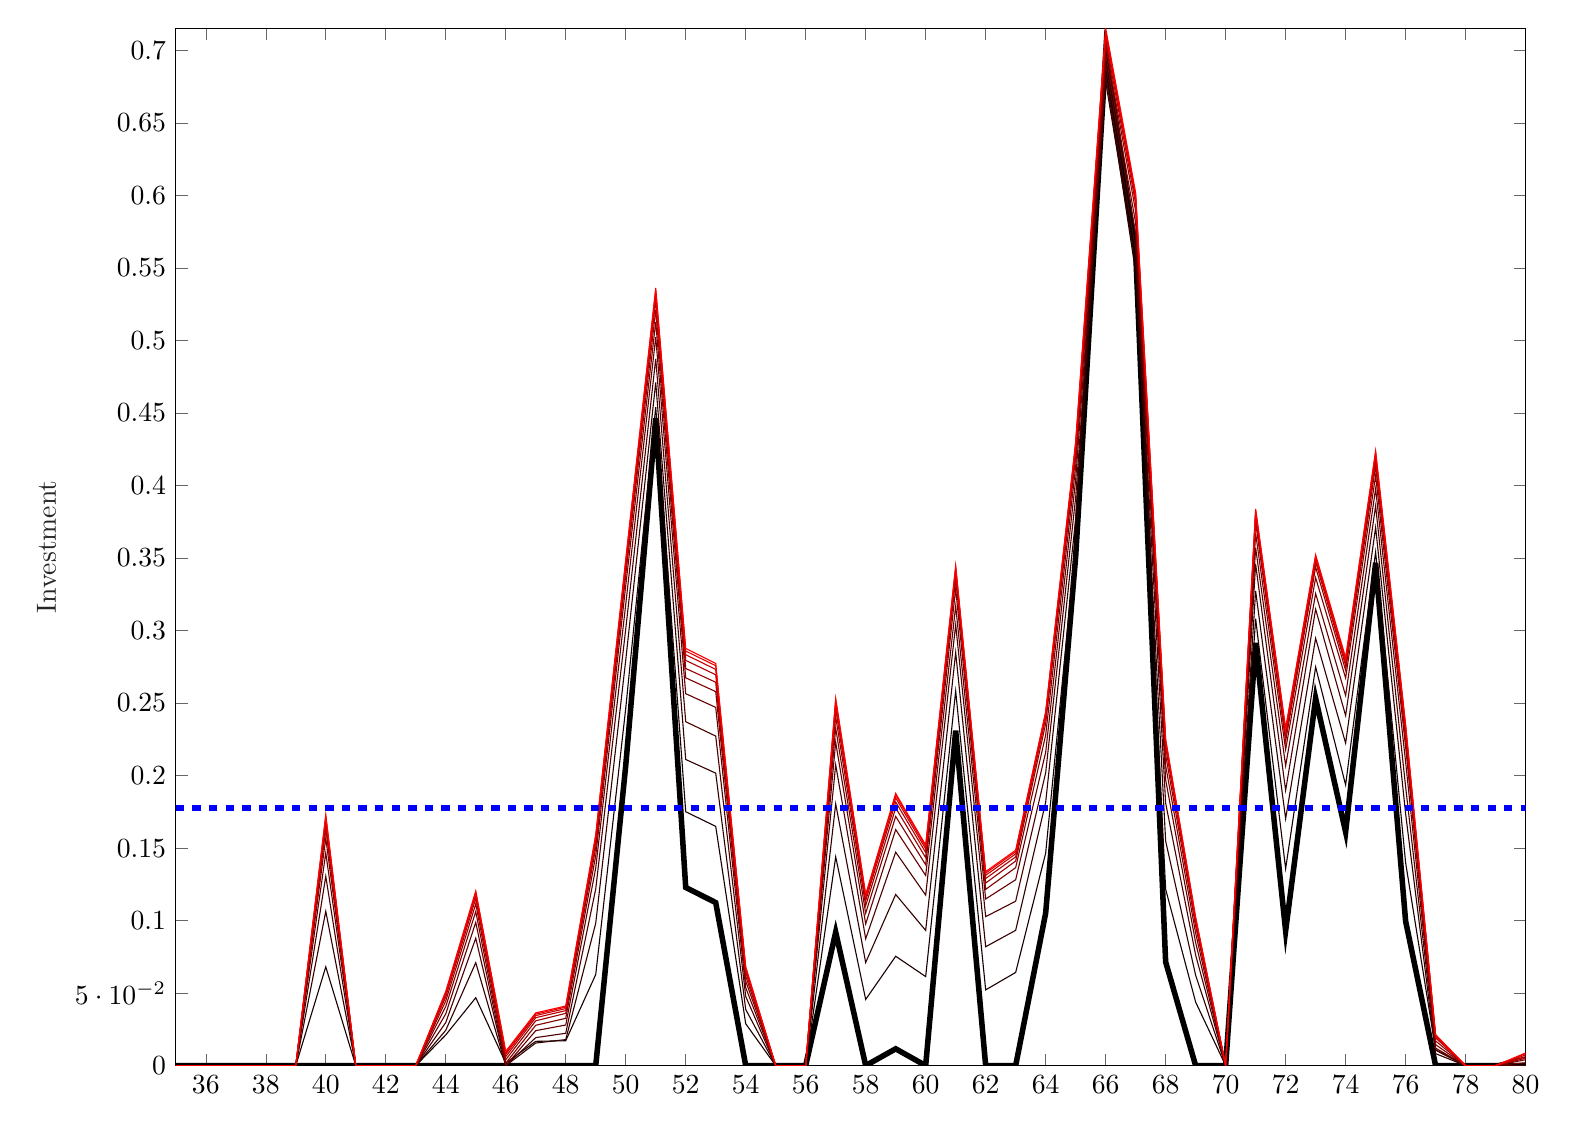
\begin{tikzpicture}

\begin{axis}[%
width=6.749in,
height=5.187in,
at={(1.132in,0.7in)},
scale only axis,
xmin=35,
xmax=80,
ymin=0,
ymax=0.715361118899045,
ylabel style={font=\color{white!15!black}},
ylabel={Investment},
axis background/.style={fill=white}
]
\addplot [color=black, line width=2.0pt, forget plot]
  table[row sep=crcr]{%
35	0\\
36	0\\
37	0\\
38	0\\
39	0\\
40	0\\
41	0\\
42	0\\
43	0\\
44	0\\
45	0\\
46	0\\
47	0\\
48	0\\
49	0\\
50	0.206912758260623\\
51	0.446325986384799\\
52	0.122858913259821\\
53	0.112422666773611\\
54	0\\
55	0\\
56	0\\
57	0.0920177891448049\\
58	0\\
59	0.011594070835933\\
60	0\\
61	0.230954610167834\\
62	0\\
63	0\\
64	0.105162150840503\\
65	0.351010667395535\\
66	0.697319916241752\\
67	0.561591796942152\\
68	0.0714783607376064\\
69	0\\
70	0\\
71	0.29145837619945\\
72	0.092956919383731\\
73	0.253298190701511\\
74	0.161126885973881\\
75	0.346750552117695\\
76	0.0996759714893127\\
77	0\\
78	0\\
79	0\\
80	0\\
};
\addplot [color=black!90!red, forget plot]
  table[row sep=crcr]{%
35	0\\
36	0\\
37	0\\
38	0\\
39	0\\
40	0.0681117903625863\\
41	0\\
42	0\\
43	0\\
44	0.0211613921163292\\
45	0.0468116052971943\\
46	0.00174778893469085\\
47	0.0167505358964546\\
48	0.0171504739568578\\
49	0.0628220730225133\\
50	0.246277837311223\\
51	0.454057133729556\\
52	0.175063423609477\\
53	0.164963941982203\\
54	0.0288731586179249\\
55	0\\
56	0\\
57	0.143934615686223\\
58	0.0456380019371685\\
59	0.0754148804910108\\
60	0.0613860656362135\\
61	0.258300586553547\\
62	0.0522360885943402\\
63	0.0642563148042232\\
64	0.146501697112415\\
65	0.359279202238604\\
66	0.683995715250124\\
67	0.547052793643154\\
68	0.121623973559258\\
69	0.0438107636106251\\
70	0\\
71	0.308193714081061\\
72	0.135786573358104\\
73	0.27486393567591\\
74	0.193560518623753\\
75	0.354145849432735\\
76	0.139943358247126\\
77	0.0109334954315852\\
78	0\\
79	0.00100154827092602\\
80	0.00600592689758072\\
};
\addplot [color=black!80!red, forget plot]
  table[row sep=crcr]{%
35	0\\
36	0\\
37	0\\
38	0\\
39	0\\
40	0.106415674835447\\
41	0\\
42	0\\
43	0\\
44	0.024357671220949\\
45	0.0709779331016356\\
46	0\\
47	0.0155765518773743\\
48	0.0179566611977335\\
49	0.0982137322709781\\
50	0.279523616110176\\
51	0.471032143738487\\
52	0.211104054377548\\
53	0.201690933048751\\
54	0.0387832717251009\\
55	0\\
56	0\\
57	0.180446972053508\\
58	0.0710951693201462\\
59	0.118020937927589\\
60	0.0932402412345885\\
61	0.284911045410003\\
62	0.0819903724304649\\
63	0.0932905783325557\\
64	0.181517486748944\\
65	0.376956529871418\\
66	0.678584457316284\\
67	0.553032382683017\\
68	0.154829196092543\\
69	0.0622915641080801\\
70	0\\
71	0.327287056516688\\
72	0.170291524851922\\
73	0.294658100368522\\
74	0.222369772600672\\
75	0.371162083772933\\
76	0.1736755781056\\
77	0.00827869683357418\\
78	0\\
79	0\\
80	0\\
};
\addplot [color=black!70!red, forget plot]
  table[row sep=crcr]{%
35	0\\
36	0\\
37	0\\
38	0\\
39	0\\
40	0.130567677969462\\
41	0\\
42	0\\
43	0\\
44	0.0297071418210097\\
45	0.0878822626507329\\
46	0\\
47	0.0193103489945729\\
48	0.0223000772109851\\
49	0.121794813254912\\
50	0.301037918300028\\
51	0.487392306532769\\
52	0.23713776855326\\
53	0.227245833447838\\
54	0.0477277973021204\\
55	0\\
56	0\\
57	0.207439916375051\\
58	0.0874617429940212\\
59	0.147187208463223\\
60	0.117586627719436\\
61	0.304019987424648\\
62	0.102726993219542\\
63	0.113372670178651\\
64	0.201917569569957\\
65	0.391758030661213\\
66	0.682796091913215\\
67	0.562759322317173\\
68	0.180991370691665\\
69	0.076224303094289\\
70	0\\
71	0.345782773683825\\
72	0.189793058582534\\
73	0.31473693305071\\
74	0.241368580534322\\
75	0.385924022227085\\
76	0.192348267056184\\
77	0.0105844125157071\\
78	0\\
79	0\\
80	0\\
};
\addplot [color=black!60!red, forget plot]
  table[row sep=crcr]{%
35	0\\
36	0\\
37	0\\
38	0\\
39	0\\
40	0.146671753310933\\
41	0\\
42	0\\
43	0\\
44	0.0357024924667959\\
45	0.0987760043408454\\
46	0\\
47	0.0241251911748879\\
48	0.027997243148399\\
49	0.136280111876889\\
50	0.318029016603176\\
51	0.502302022382199\\
52	0.256481362991278\\
53	0.247042304676943\\
54	0.0537616353671089\\
55	0\\
56	0\\
57	0.222964053904698\\
58	0.0976889943670942\\
59	0.16275053739878\\
60	0.131104163639335\\
61	0.316935160005611\\
62	0.114918495259294\\
63	0.128180461793758\\
64	0.216038840222609\\
65	0.403984570505078\\
66	0.690096041887973\\
67	0.573756188481209\\
68	0.19716914378205\\
69	0.0847648058718482\\
70	0\\
71	0.357090280730415\\
72	0.206774785429782\\
73	0.325510121945014\\
74	0.255194671105243\\
75	0.397766950819866\\
76	0.209347379324695\\
77	0.0120893172341192\\
78	0\\
79	0\\
80	0.00201275192076444\\
};
\addplot [color=black!50!red, forget plot]
  table[row sep=crcr]{%
35	0\\
36	0\\
37	0\\
38	0\\
39	0\\
40	0.156805282544082\\
41	0\\
42	0\\
43	0\\
44	0.0407708586422433\\
45	0.106188669069305\\
46	0.00171496688099482\\
47	0.0278143805307367\\
48	0.0326170948581634\\
49	0.144748863970502\\
50	0.330817710196351\\
51	0.512700381535334\\
52	0.267414160107469\\
53	0.2579036881991\\
54	0.0582922704132751\\
55	0\\
56	0\\
57	0.232637733832658\\
58	0.105078400597791\\
59	0.171803513239536\\
60	0.13852039136386\\
61	0.328809071735712\\
62	0.121540001705527\\
63	0.136513318014999\\
64	0.227867158290283\\
65	0.413034548798028\\
66	0.697014761232125\\
67	0.581135601864793\\
68	0.206875821453857\\
69	0.0913022657241946\\
70	0\\
71	0.366974267830061\\
72	0.217908514772061\\
73	0.336437647755389\\
74	0.267245179849641\\
75	0.406862168744479\\
76	0.219791063376011\\
77	0.0144770613395519\\
78	0\\
79	0\\
80	0.00405573043783769\\
};
\addplot [color=black!40!red, forget plot]
  table[row sep=crcr]{%
35	0\\
36	0\\
37	0\\
38	0\\
39	0\\
40	0.16313999990383\\
41	0\\
42	0\\
43	0\\
44	0.0446181696475938\\
45	0.111471169215879\\
46	0.00409999395808902\\
47	0.0309134592287361\\
48	0.0360351047074721\\
49	0.150194462656308\\
50	0.33813302237664\\
51	0.520963821800648\\
52	0.273874681479601\\
53	0.264375892426975\\
54	0.0617791778645535\\
55	0\\
56	0\\
57	0.240485313501495\\
58	0.110320102225508\\
59	0.17765600306589\\
60	0.14341492657476\\
61	0.335999332185346\\
62	0.125885365660744\\
63	0.141092910282964\\
64	0.23582332632736\\
65	0.419752322871557\\
66	0.703247801163574\\
67	0.589100759247454\\
68	0.214321281191051\\
69	0.0960710058380955\\
70	0\\
71	0.37452101378913\\
72	0.22366795095235\\
73	0.34368077712592\\
74	0.272605666126184\\
75	0.413541253511453\\
76	0.225125427404395\\
77	0.0170056142715214\\
78	0\\
79	0\\
80	0.00505602069957911\\
};
\addplot [color=black!30!red, forget plot]
  table[row sep=crcr]{%
35	0\\
36	0\\
37	0\\
38	0\\
39	0\\
40	0.167106633140723\\
41	0\\
42	0\\
43	0\\
44	0.0474068035601009\\
45	0.115222224235801\\
46	0.00621326584703019\\
47	0.0330521860924273\\
48	0.0379466803977728\\
49	0.153903751673674\\
50	0.342567131833056\\
51	0.527413519205792\\
52	0.279431096747759\\
53	0.269534512872381\\
54	0.064464213757504\\
55	0\\
56	0\\
57	0.245944125315474\\
58	0.113772459955472\\
59	0.181788270882988\\
60	0.146974091256365\\
61	0.339810732425141\\
62	0.129009586130059\\
63	0.143934130326027\\
64	0.239728818653802\\
65	0.424078831734667\\
66	0.70746191740563\\
67	0.594326956063375\\
68	0.219434715754488\\
69	0.0987954211360202\\
70	0\\
71	0.37860148373816\\
72	0.226806608296756\\
73	0.347323250675835\\
74	0.27588800771343\\
75	0.417586343632361\\
76	0.228727854403403\\
77	0.0190873318372542\\
78	0\\
79	0\\
80	0.00600729683528844\\
};
\addplot [color=black!20!red, forget plot]
  table[row sep=crcr]{%
35	0\\
36	0\\
37	0\\
38	0\\
39	0\\
40	0.169962364787538\\
41	0\\
42	0\\
43	0\\
44	0.0492572621046447\\
45	0.11769929439943\\
46	0.00786386236738789\\
47	0.0345066825826126\\
48	0.0393439735382426\\
49	0.156394485509749\\
50	0.345434255142012\\
51	0.531621196009331\\
52	0.283353478930727\\
53	0.273215401771478\\
54	0.0663232055037659\\
55	0\\
56	0\\
57	0.249486570269065\\
58	0.11585459285615\\
59	0.184614121543195\\
60	0.149398525888008\\
61	0.342053294515015\\
62	0.131198579663252\\
63	0.146012816133238\\
64	0.241957817213452\\
65	0.426977147533611\\
66	0.711118527392388\\
67	0.597661867808498\\
68	0.222636359640798\\
69	0.100601499795512\\
70	0\\
71	0.380954565942905\\
72	0.229339958317151\\
73	0.349360797519566\\
74	0.277964845214992\\
75	0.420599050758286\\
76	0.231864534311277\\
77	0.020268730525538\\
78	0\\
79	0\\
80	0.00727348087991375\\
};
\addplot [color=black!10!red, forget plot]
  table[row sep=crcr]{%
35	0\\
36	0\\
37	0\\
38	0\\
39	0\\
40	0.171754039392575\\
41	0\\
42	0\\
43	0\\
44	0.0503797527646557\\
45	0.119467524317999\\
46	0.0090473167315479\\
47	0.0355124377090945\\
48	0.0403539542536082\\
49	0.158132511646645\\
50	0.347545973602497\\
51	0.53451812252946\\
52	0.285885742581521\\
53	0.275770557553196\\
54	0.0674876738314587\\
55	0\\
56	0\\
57	0.251799535841536\\
58	0.117208647256008\\
59	0.186484128855344\\
60	0.151026359580838\\
61	0.34356877009719\\
62	0.132733112855797\\
63	0.147511553702\\
64	0.243213266029993\\
65	0.42907897059573\\
66	0.713515957044485\\
67	0.600039380584835\\
68	0.224262732580199\\
69	0.101645463698508\\
70	0\\
71	0.38262094674385\\
72	0.231327629635072\\
73	0.350979415322803\\
74	0.279884412095189\\
75	0.422627242444269\\
76	0.233977738992102\\
77	0.0209295810047918\\
78	0\\
79	0\\
80	0.00821650206871016\\
};
\addplot [color=red, forget plot]
  table[row sep=crcr]{%
35	0\\
36	0\\
37	0\\
38	0\\
39	0\\
40	0.172857147597689\\
41	0\\
42	0\\
43	0\\
44	0.0511981633671694\\
45	0.120414815350031\\
46	0.00988874687401652\\
47	0.0363732749912582\\
48	0.0410795750627948\\
49	0.159266049313152\\
50	0.349092388353274\\
51	0.536199621222013\\
52	0.287665730745454\\
53	0.277353792515928\\
54	0.0682028962300156\\
55	0\\
56	0\\
57	0.253309749789706\\
58	0.117966836307206\\
59	0.187725128407274\\
60	0.15213452648711\\
61	0.344730219048969\\
62	0.13376723076841\\
63	0.148535751958996\\
64	0.243970559582037\\
65	0.430317645662782\\
66	0.715361118899045\\
67	0.601935680318696\\
68	0.225150094156996\\
69	0.102312025334615\\
70	0\\
71	0.383907543893641\\
72	0.232648362342682\\
73	0.352198304957331\\
74	0.281399568372125\\
75	0.423967091714583\\
76	0.235363236901556\\
77	0.0213938703037113\\
78	0\\
79	0\\
80	0.00873377852301238\\
};
\addplot [color=blue, dashed, line width=2.0pt, forget plot]
  table[row sep=crcr]
  \end{center}

\end{frame}


\end{document}
